\graphicspath{{figuras/}{./figuras/}}

\chapter[Gráficos, escalas e percepção]{Gráficos, escalas e percepção: escolher pela pergunta}

\section{O mesmo resultado, duas histórias visuais}

Uma central de atendimento fechou agosto com tempo mediano de espera de 4,8 minutos, diante de uma meta de 5 minutos. A frase ``a meta foi cumprida'' é verdadeira, mas ainda não informa se a operação melhorou, se todos os turnos melhoraram ou se poucos dias excepcionais esconderam uma semana crítica. Uma tabela com o único valor 4,8 permite verificar o indicador; um gráfico pode revelar sua estrutura. O ponto de partida deste capítulo é que visualizar não significa decorar números. Significa construir uma representação que torne uma pergunta mais fácil de responder sem deformar o dado.

Considere a série mensal 5,1; 5,0; 4,9; 4,8. Em um gráfico cujo eixo vertical vai de zero a dez, a queda parece discreta. Se o eixo começa em 4,7 e termina em 5,2, a mesma queda ocupa quase toda a altura e parece dramática. Nenhum ponto mudou. Mudou a razão visual entre a diferença observada e o espaço disponível. A primeira versão pode esconder uma variação operacional relevante; a segunda pode exagerá-la. O analista responsável mostra a escala, explica o propósito e oferece contexto suficiente para que a leitura não dependa de um recorte conveniente.

Antes de escolher ``barras ou linhas'', formule a tarefa. Perguntas como ``qual turno espera mais?'', ``a espera está caindo?'', ``como os atendimentos se distribuem?'', ``volume e espera caminham juntos?'' e ``qual canal compõe o total?'' pedem operações perceptivas diferentes. Elas correspondem, respectivamente, a comparação, tendência, distribuição, relação e composição. O tipo de gráfico é consequência dessa operação. Começar pela galeria da ferramenta costuma produzir uma resposta visualmente atraente para uma pergunta que ninguém fez.

Chamaremos de marca o elemento geométrico que representa uma observação ou agregado: ponto, linha, barra ou área. Chamaremos de canal visual a propriedade que codifica um valor: posição, comprimento, inclinação, área, cor, forma ou tamanho. Essa linguagem de marcas e canais organiza escolhas visuais de forma sistemática e aparece tanto na gramática dos gráficos quanto em abordagens modernas de projeto de visualização \cite{wilkinson2005,munzner2014}. Uma barra usa posição e comprimento; um diagrama de dispersão usa duas posições; um mapa coroplético usa cor sobre áreas geográficas. O gráfico é, portanto, uma função que transforma campos do conjunto de dados em marcas e canais sob uma escala definida.

Essa transformação carrega decisões. Agregar pela média ou pela mediana, ordenar por valor ou alfabeticamente, mostrar taxa ou contagem, conservar zero ou ampliar uma faixa, separar turnos ou misturá-los: tudo isso antecede fonte, legenda e paleta. Um gráfico correto precisa respeitar o contrato semântico construído nos capítulos anteriores. Se o grão contém uma linha por atendimento, a taxa diária exige numerador e denominador diários; somar percentuais de linhas diferentes não cria uma taxa válida.

Ao final deste capítulo, a pergunta continua sendo o teste principal: que comparação o leitor precisa executar e quanto esforço a representação impõe? A resposta deverá mencionar unidade, população, período, agregação, escala, incerteza e limite de interpretação. Matplotlib, seaborn, Tableau, Power BI ou outra ferramenta podem implementar essa decisão, mas não a substituem. O caso da central será retomado para mostrar que uma boa escolha visual é uma hipótese verificável sobre como o leitor perceberá a evidência.

\begin{SummaryBox}
\textbf{Regra de trabalho.} Escreva primeiro uma frase no formato ``preciso comparar \emph{X} entre \emph{Y} para decidir \emph{Z}''. Só depois escolha marcas, canais, escala e anotações. Se o gráfico não torna essa comparação mais direta, redesenhe-o.
\end{SummaryBox}



\begin{figure}[H]
\centering
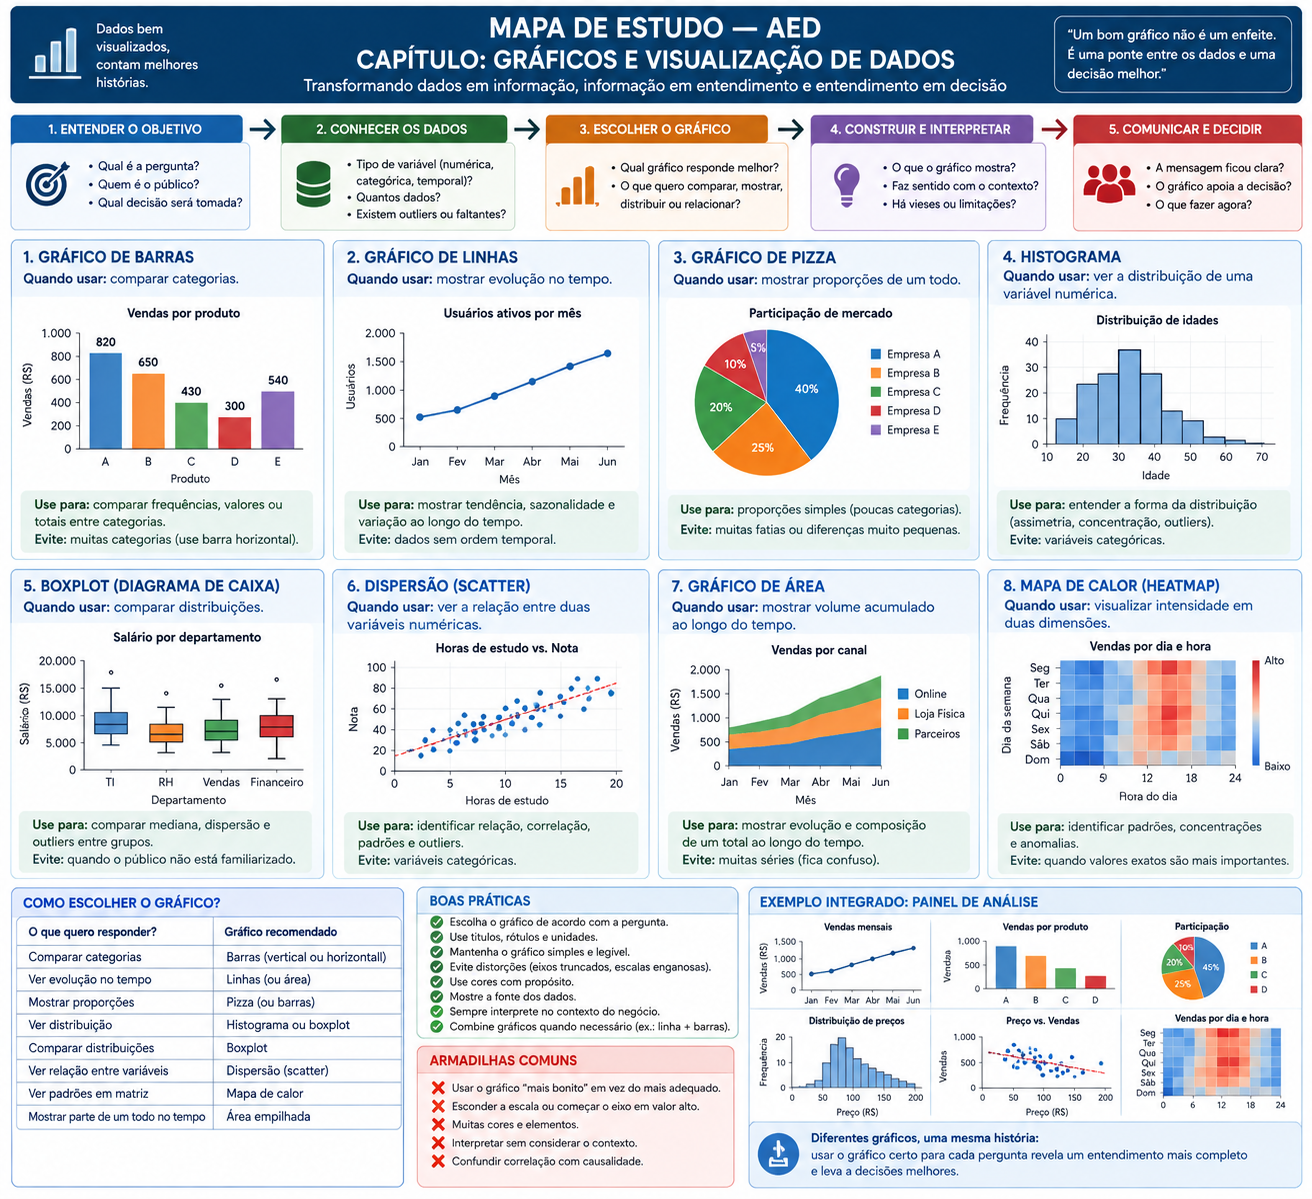
\includegraphics[width=0.96\textwidth]{mapa_cap06_graficos.png}
\caption{Mapa do capítulo: a escolha do gráfico começa pela pergunta, passa pelo tipo de dado e pela tarefa perceptiva, e termina em uma decisão comunicável. A imagem funciona como visão geral; as seções seguintes desmontam cada escolha e mostram exemplos com dados.}
\label{fig:mapa-cap06}
\end{figure}

A Figura~\ref{fig:mapa-cap06} deve ficar visível no início da aula. Ela não é uma tabela de receitas universais. É um mapa de perguntas. A primeira coluna pergunta o que precisa ser decidido; a segunda obriga o analista a reconhecer tipo de variável, grão e qualidade; a terceira oferece famílias de gráficos; a quarta lembra que a construção precisa ser interpretada; a quinta devolve a representação ao contexto. Essa sequência é coerente com a ideia de abstrair primeiro os dados e a tarefa para depois selecionar marcas e canais \cite{munzner2014}. A gramática de Wilkinson também ajuda a enxergar gráfico como composição de dados, transformações, escalas e elementos geométricos, e não como um objeto fechado escolhido em um menu \cite{wilkinson2005}.

\begin{center}
\small
\begin{tabularx}{0.96\textwidth}{p{3.2cm} p{2.3cm} X X}
\toprule
\textbf{Pergunta principal} & \textbf{Operação} & \textbf{Primeira escolha} & \textbf{Atenção / quando trocar} \\
\midrule
Qual categoria é maior ou menor? & comparação & barras ou pontos ordenados & se valores exatos importam, acompanhe com tabela; se há antes/depois, use pontos conectados \\
Como a métrica evolui? & tendência & linha temporal & respeite lacunas, granularidade e eventos; não ligue categorias nominais \\
Como os valores se espalham? & distribuição & histograma; boxplot entre grupos & histograma mostra forma; boxplot resume e facilita comparação, mas esconde multimodalidade \\
Duas variáveis caminham juntas? & relação & dispersão & procure forma, grupos e outliers antes de calcular correlação; associação não prova causa \\
Como o total se divide? & composição & barra empilhada / 100\%; barras para comparação precisa & setor serve apenas para poucas partes grosseiramente distintas; preserve denominador \\
Onde e quando há concentração? & padrão em matriz & heatmap & cor precisa de legenda e escala; não use se o valor exato é a tarefa principal \\
Quanto sabemos sobre a estimativa? & incerteza & ponto + intervalo / faixa & informe método, $n$, nível e suposições; barra de erro não é teste automático \\
\bottomrule
\end{tabularx}
\end{center}

A tabela anterior é o primeiro instrumento prático do capítulo. Ela transforma ``qual gráfico eu uso?'' em ``qual operação o leitor precisa executar?''. Essa mudança é importante porque a mesma tabela de dados pode sustentar gráficos diferentes, cada um correto para uma tarefa diferente. Um histograma e um boxplot podem usar exatamente a mesma coluna de tempos, porém o primeiro favorece leitura da forma e o segundo favorece comparação compacta entre grupos. Um gráfico de linhas e um conjunto de barras podem usar os mesmos totais mensais, porém a linha enfatiza continuidade e a barra enfatiza comparação de magnitudes discretas. Escolher gráfico é escolher qual comparação ficará mais fácil.

A primeira demonstração deve ocorrer antes de discutir tipos específicos. A Figura~\ref{fig:eixo-amplo}, nos painéis (a) e (b), usa os mesmos quatro valores mensais. O objetivo é mostrar que o dado não ``fala sozinho'': escala, proporção do painel e marca influenciam a percepção. A literatura de percepção gráfica nasceu justamente da tentativa de estudar como pessoas decodificam visualmente quantidades e comparações \cite{cleveland1984,heer2010}. Em sala, peça aos alunos que descrevam a tendência sem mostrar os valores; depois revele que ambos os gráficos representam a mesma série.

\begin{figure}[H]
\centering
\begin{minipage}[t]{0.48\textwidth}
\centering
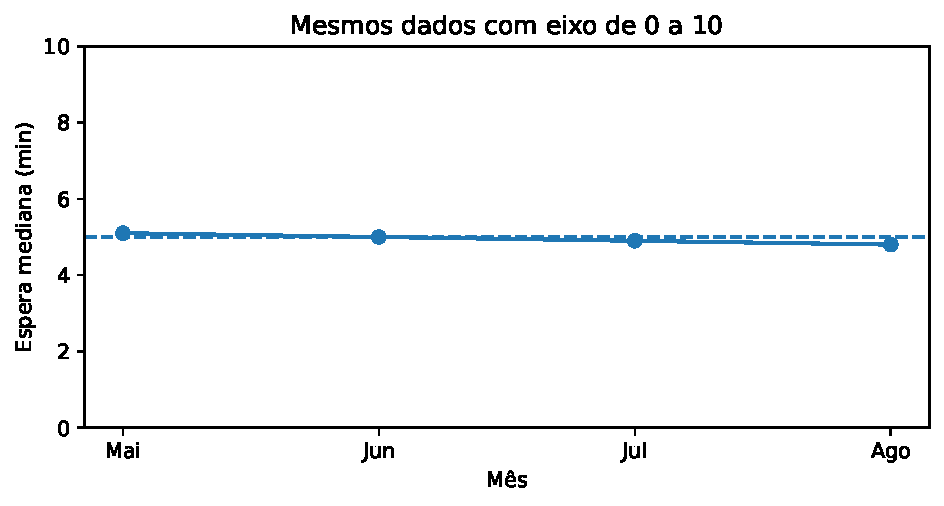
\includegraphics[width=\linewidth]{fig_06_01a_escala_ampla.pdf}
\caption*{(a) Eixo amplo: a queda parece pequena.}
\end{minipage}\hfill
\begin{minipage}[t]{0.48\textwidth}
\centering
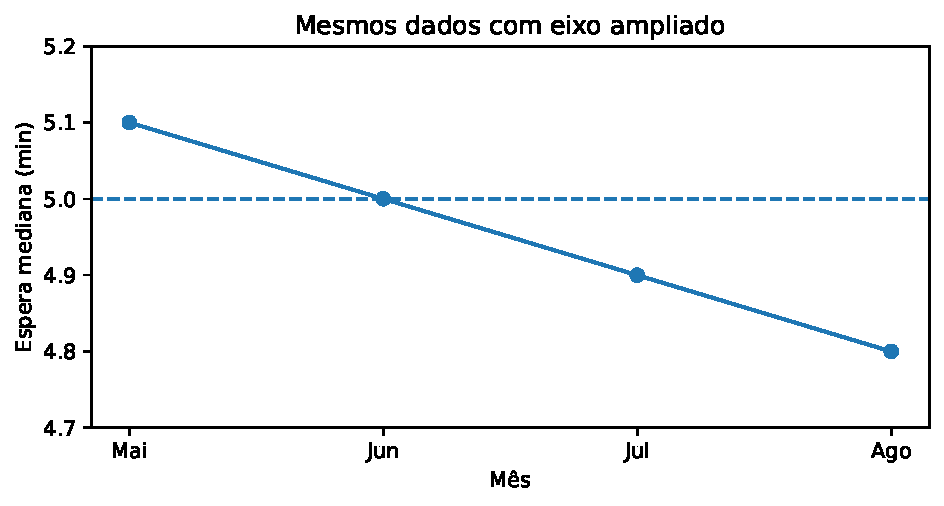
\includegraphics[width=\linewidth]{fig_06_01b_escala_zoom.pdf}
\caption*{(b) Eixo ampliado: a mesma queda ocupa quase todo o painel.}
\end{minipage}
\caption{Mesmos dados, duas histórias visuais possíveis. O recorte pode ser legítimo em linhas e pontos, mas precisa estar visível e ser interpretado em unidade real. \FonteDidatica}
\label{fig:eixo-amplo}
\label{fig:eixo-zoom}
\end{figure}

\begin{GuidedBox}
\textbf{Pergunta para a turma.} O gráfico da direita está ``errado''? A resposta esperada é: não automaticamente. Como a linha codifica valor principalmente por posição, ampliar o eixo pode ajudar a investigar pequenas variações; o problema surge quando o recorte é escondido ou quando a narrativa transforma uma diferença pequena em efeito substantivamente enorme. Em barras, cortar a base é muito mais problemático porque o comprimento desde a base é parte da codificação. A pergunta correta é sempre: \emph{o que a distância visual significa neste gráfico?}
\end{GuidedBox}


\section{Comparação: posição e comprimento antes do enfeite}

Para comparar categorias, uma tabela é excelente quando o leitor precisa recuperar valores exatos. Um gráfico de barras é superior quando precisa perceber rapidamente ordem, distância e exceções. Suponha medianas de espera por turno: manhã 3,9, tarde 5,7, noite 4,6 e madrugada 6,2 minutos. Ordenadas do maior para o menor, as barras respondem de imediato onde agir. Em ordem alfabética, o leitor precisa saltar entre posições para reconstruir o ranking. Ordenar é uma decisão analítica, não apenas estética.

A precisão vem do canal. Experimentos clássicos e replicações posteriores mostram que tarefas baseadas em posição sobre escala comum tendem a permitir julgamentos quantitativos mais precisos do que tarefas baseadas em ângulo ou área \cite{cleveland1984,heer2010,zeng2023}. Por isso, pontos alinhados e barras tendem a favorecer comparação quantitativa. Comprimentos também são eficazes quando partem da mesma base. Já círculos proporcionais exigem estimar área: para representar o dobro do valor, o raio deve crescer por $\sqrt{2}$, não por dois. Se dobrarmos o raio, a área quadruplica e a percepção induz uma diferença inexistente.

Em barras, o zero é parte da gramática porque o comprimento codifica o valor. Cortar a base de 0 para 5 em valores 5,7 e 6,2 faz a segunda barra parecer quase três vezes maior, embora a razão real seja $6{,}2/5{,}7\approx1{,}09$. Para pontos ou linhas, a posição, e não o comprimento desde zero, carrega a medida; um recorte pode ser legítimo para examinar pequena variação, desde que o eixo esteja visível e o contexto seja declarado. A regra não é ``todo eixo começa em zero'', mas ``não mude a operação perceptiva sem avisar''.

Quando há duas condições, barras agrupadas funcionam para poucas categorias, mas ficam congestionadas rapidamente. Um gráfico de pontos conectados pode mostrar antes e depois: cada turno recebe dois pontos na mesma linha e a inclinação revela direção. Se manhã cai de 5,2 para 3,9 e madrugada sobe de 5,8 para 6,2, a representação destaca movimentos opostos que duas colunas de números esconderiam. Para muitas categorias, pequenos múltiplos ou uma matriz podem reduzir o esforço de procurar cores em uma legenda distante.

Uma comparação responsável inclui denominadores. Dizer que a madrugada teve 18 reclamações e a manhã 30 sugere pior desempenho matinal. Se houve 300 atendimentos na madrugada e 2.000 pela manhã, as taxas são 6\% e 1,5\%. Contagem responde a carga absoluta; taxa responde a risco relativo. Ambas podem ser necessárias, lado a lado, com unidades explícitas. Escolher uma sem declarar a decisão pode deslocar recursos para o lugar errado.

O título também participa da análise. ``Espera por turno'' nomeia o assunto; ``Madrugada excede a meta apesar do menor volume'' explicita a descoberta verificável. O segundo não deve afirmar causa nem substituir a leitura dos dados. Uma linha de meta em 5 minutos, rótulos apenas nos extremos e uma nota sobre o período completam a evidência. Bordas, sombras e ícones não melhoram a comparação; em excesso, competem com os sinais que deveriam orientar o olhar.

\begin{center}
\begin{tabular}{lrrr}
\toprule
Turno & Atendimentos & Reclamações & Taxa \\
\midrule
Manhã & 2.000 & 30 & 1,5\% \\
Tarde & 1.400 & 35 & 2,5\% \\
Noite & 800 & 28 & 3,5\% \\
Madrugada & 300 & 18 & 6,0\% \\
\bottomrule
\end{tabular}
\end{center}



A Figura~\ref{fig:barras-turnos} transforma as quatro medianas de espera em uma comparação ordenada. O eixo horizontal começa em zero porque o comprimento da barra representa magnitude. A linha de cinco minutos adiciona o contexto decisório: não basta saber quem é maior; interessa saber quem ultrapassa a meta. Em vez de memorizar ``barras para categorias'', o aluno deve associar barras à tarefa de comparar comprimentos a partir de uma base comum. Essa escolha é particularmente forte quando categorias são nominais ou ordinais e a magnitude é a principal pergunta \cite{cleveland1984,few2012,wilke2019}.

\begin{figure}[H]
\centering
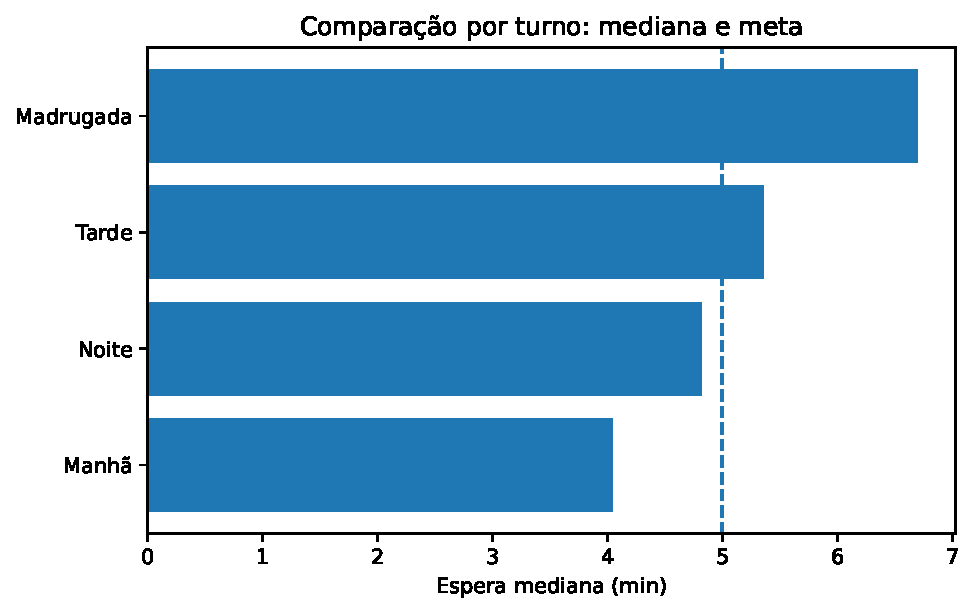
\includegraphics[width=0.76\textwidth]{fig_06_02_barras_turnos.pdf}
\caption{Barras horizontais ordenadas tornam ranking e distância para a meta imediatamente visíveis. \FonteDidatica}
\label{fig:barras-turnos}
\end{figure}

Há, entretanto, duas perguntas muito parecidas que exigem denominadores diferentes. A Figura~\ref{fig:contagem-reclamacoes}, nos painéis (a) e (b), usa as mesmas reclamações. A primeira pergunta ``onde há mais reclamações em número absoluto?''; a segunda pergunta ``em qual turno a reclamação é mais provável por atendimento?''. No caso didático, a madrugada tem volume total muito menor, mas taxa muito maior. Se a decisão é dimensionar uma equipe para tratar tickets, a contagem pode importar. Se a decisão é corrigir uma experiência ruim, a taxa oferece outra evidência. Não existe conflito entre os gráficos; existem perguntas distintas.

\begin{figure}[H]
\centering
\begin{minipage}[t]{0.48\textwidth}
\centering
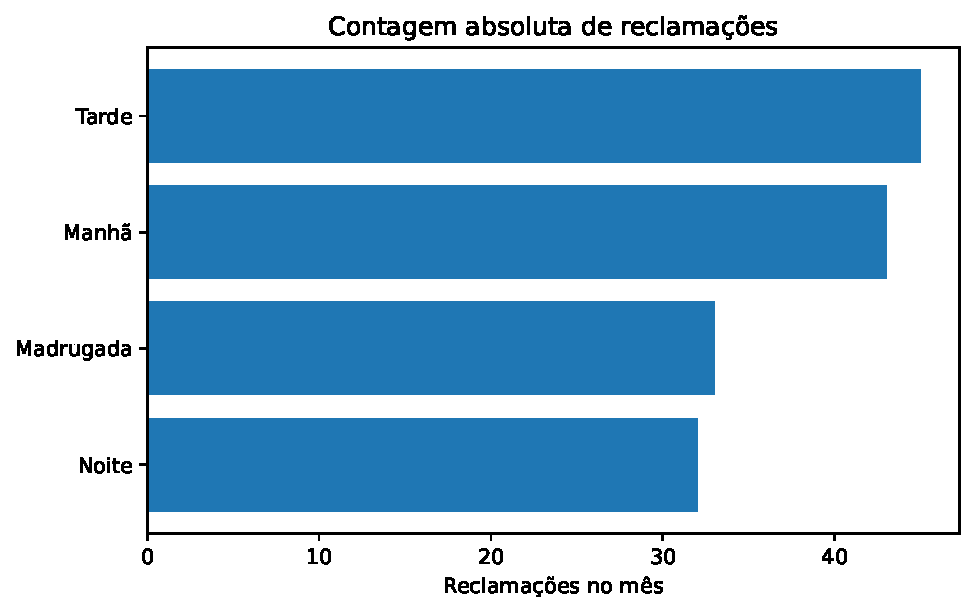
\includegraphics[width=\linewidth]{fig_06_03a_contagem_reclamacoes.pdf}
\caption*{(a) Carga absoluta.}
\end{minipage}\hfill
\begin{minipage}[t]{0.48\textwidth}
\centering
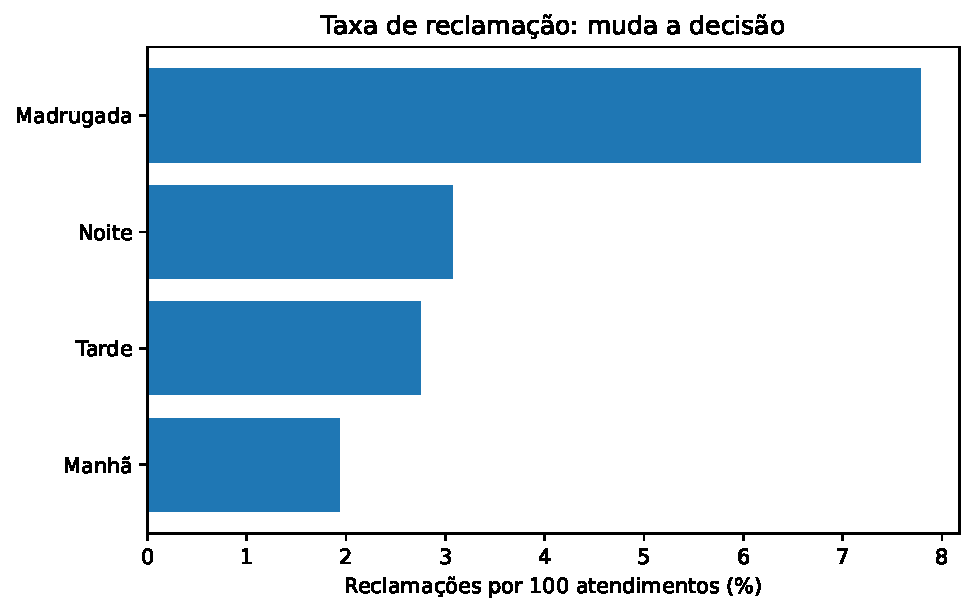
\includegraphics[width=\linewidth]{fig_06_03b_taxa_reclamacoes.pdf}
\caption*{(b) Risco relativo ao volume.}
\end{minipage}
\caption{Contagem e taxa respondem perguntas diferentes. Um gráfico só é interpretável quando o denominador está claro. \FonteDidatica}
\label{fig:contagem-reclamacoes}
\label{fig:taxa-reclamacoes}
\end{figure}

Quando a pergunta é mudança entre duas condições, duas barras por categoria funcionam, mas obrigam o leitor a comparar alturas e procurar cores. O gráfico de pontos conectados da Figura~\ref{fig:antes-depois} mantém cada turno em uma linha e transforma a distância entre pontos na mudança. Essa construção é útil para antes/depois, planejado/realizado, grupo A/grupo B ou duas versões de um sistema. O segmento conecta condições comparáveis; ele não implica que conhecemos a trajetória intermediária.

\begin{figure}[H]
\centering
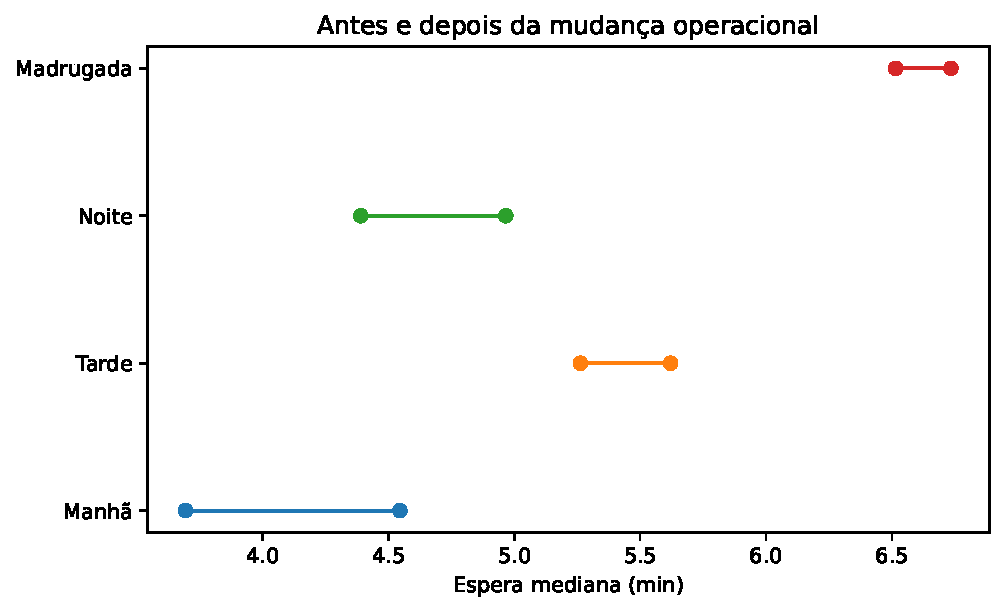
\includegraphics[width=0.74\textwidth]{fig_06_04_antes_depois.pdf}
\caption{Pontos conectados: alternativa compacta a barras agrupadas quando existem apenas duas condições por categoria. \FonteDidatica}
\label{fig:antes-depois}
\end{figure}

\begin{GuidedBox}
\textbf{Escolha rápida para comparação.} Use \textbf{barras} quando o comprimento desde zero é uma metáfora natural da magnitude; use \textbf{pontos} quando a posição basta e o zero não precisa dominar o espaço; use \textbf{pontos conectados} para duas condições; use \textbf{tabela} quando a tarefa é recuperar números exatos. Antes de publicar, pergunte: a ordem ajuda a decisão? o denominador está explícito? a base das barras é zero? a meta ou referência necessária aparece?
\end{GuidedBox}


\section{Tendência: tempo, continuidade e contexto}

Uma linha conecta observações e sugere continuidade. Ela é adequada quando o eixo horizontal tem ordem temporal ou outra sequência significativa. Trocar a ordem dos meses mudaria a história; trocar a ordem de quatro categorias não altera sua identidade. Essa diferença explica por que ligar categorias nominais com linhas é perigoso: o segmento inventa uma transição que o dado não possui. Em uma série temporal, a conexão orienta a leitura de nível, direção, velocidade, sazonalidade e ruptura.

O intervalo temporal altera a conclusão. Médias mensais podem esconder uma pane de três dias; valores horários podem transformar ruído em aparente urgência. Na central, a mediana mensal caiu, mas o gráfico diário revela uma fila intensa toda segunda-feira. A granularidade deve corresponder à latência da decisão: quem escala equipes diariamente precisa ver dias ou horas; quem negocia orçamento trimestral pode precisar de semanas ou meses. Agregar não é neutro, pois remove variações em nome de um padrão mais amplo.

Compare variação absoluta e relativa. Cair de 6 para 5 minutos significa menos 1 minuto e redução de $1/6\approx16{,}7\%$. Cair de 2 para 1 minuto também significa menos 1 minuto, porém 50\%. O eixo e o rótulo precisam informar qual medida orienta a decisão. Indexar séries em 100 numa data inicial ajuda a comparar ritmos de mudança entre métricas de unidades diferentes, mas apaga seus níveis originais. Um índice é útil para tendência relativa, não para afirmar que dois serviços têm o mesmo desempenho.

Linhas de referência fornecem contexto: meta, mediana histórica, limite regulatório ou início de uma intervenção. Elas devem ser semanticamente estáveis. Uma meta que muda no meio do período precisa aparecer em degraus ou segmentos, não como linha horizontal única. Anotações devem marcar eventos conhecidos sem declarar automaticamente causalidade. ``Novo roteador implantado'' é observação temporal; ``roteador reduziu a espera'' exige desenho de avaliação, grupo de comparação ou outra evidência além da coincidência.

Suavização ajuda a enxergar tendência, mas cobra transparência. Uma média móvel de sete dias substitui cada ponto pela média de uma janela. Para valores 4, 6 e 8, a média móvel simples de três períodos no centro é $(4+6+8)/3=6$. A curva suavizada reduz ruído e introduz atraso, além de perder pontos nas bordas conforme o método. Mostrar linha bruta em cinza e suavizada em destaque preserva o vínculo com observações. Ocultar a série original pode fazer uma escolha de janela parecer um fato.

Também é preciso respeitar lacunas. Conectar janeiro diretamente a março quando fevereiro está ausente sugere que houve uma trajetória observada entre os pontos. O gráfico deve interromper a linha, marcar ausência ou explicar imputação. Frequência irregular pede datas reais no eixo, não posições igualmente espaçadas. Em tempo, distância visual representa duração; falsificar o espaçamento falsifica velocidade. A leitura crítica procura esses detalhes antes de aceitar uma narrativa de crescimento ou queda.

\begin{GuidedBox}
\textbf{Leitura de uma tendência.} Procure nível, direção, variação, sazonalidade, ruptura, lacunas e janela de agregação. Depois pergunte se a escala mostra valores absolutos, percentuais, índices ou transformação logarítmica.
\end{GuidedBox}



A Figura~\ref{fig:serie-temporal} reúne quatro elementos que um gráfico de tendência pode precisar: observação diária, suavização, meta e evento conhecido. Cada camada responde a uma pergunta. Os pontos diários preservam variabilidade; a média móvel ajuda a enxergar direção; a meta permite julgar desempenho; a linha vertical marca quando uma mudança operacional ocorreu. Nenhuma dessas camadas, isoladamente, demonstra causalidade. O gráfico organiza tempo suficiente para formular perguntas mais fortes.

\begin{figure}[H]
\centering
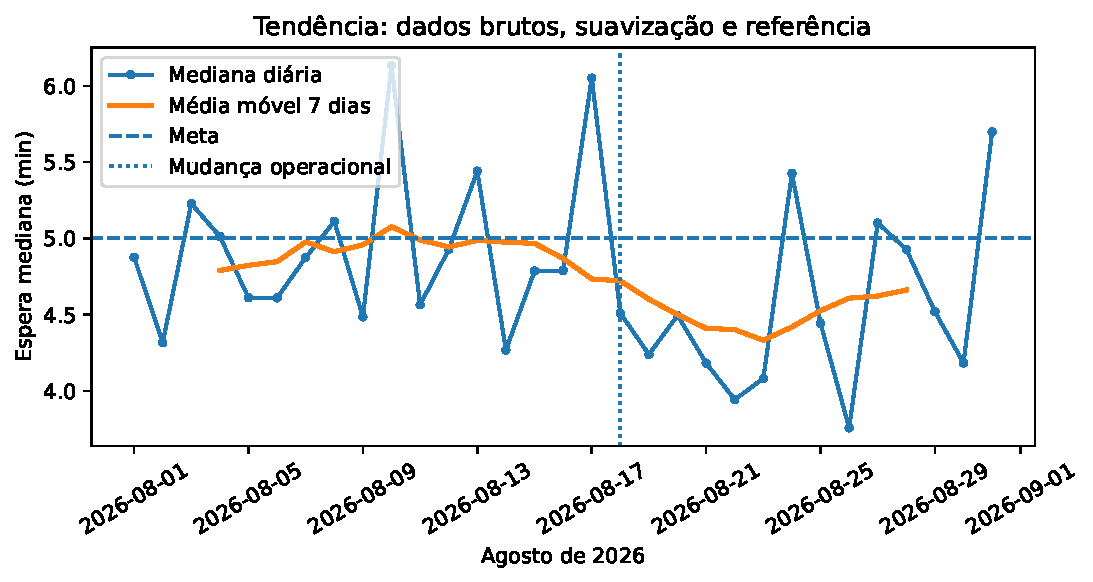
\includegraphics[width=0.88\textwidth]{fig_06_05_serie_temporal.pdf}
\caption{Série temporal com observações, suavização, meta e evento. A linha suavizada ajuda a enxergar tendência, mas a série bruta permanece visível. \FonteDidatica}
\label{fig:serie-temporal}
\end{figure}

Em aula, peça ao aluno que leia a figura em quatro passadas. Primeiro, descreva apenas o \textbf{nível}: em que faixa os valores estão? Segundo, descreva \textbf{direção e velocidade}: cresce, cai ou permanece estável? Terceiro, procure \textbf{padrões repetidos, rupturas e lacunas}. Quarto, relacione a série a referências externas, como meta ou intervenção. Esse método reduz a tendência de olhar um único ponto e declarar tendência. Ele também explica por que uma linha temporal deve preservar a ordem e o espaçamento real do tempo.

A escolha entre linha e barras no tempo depende do que se quer salientar. Se a pergunta é continuidade, trajetória ou taxa de mudança, linha é normalmente a primeira escolha. Se os períodos são poucos e independentes, como total anual em cinco anos para uma apresentação executiva, barras também podem funcionar. Para eventos discretos, pontos podem ser suficientes. Para muitas séries, sobrepor linhas cria um ``espaguete''; pequenos múltiplos, discutidos mais adiante, preservam a forma sem exigir uma legenda com dez cores \cite{wilke2019,munzner2014}.

\begin{GuidedBox}
\textbf{Pergunta para a turma.} A linha começou a cair depois de 18 de agosto. Podemos escrever ``a mudança de 18 de agosto reduziu a espera''? Não com esse gráfico sozinho. Podemos escrever que a queda ocorreu \emph{após} a mudança e que o padrão é compatível com uma melhoria. Atribuir efeito exige desenho de avaliação, controle de fatores concorrentes ou outra evidência causal.
\end{GuidedBox}


\section{Distribuição: enxergar o que a média esconde}

A média de espera pode cumprir a meta enquanto uma parcela dos clientes enfrenta atrasos extremos. Distribuição é a pergunta sobre como valores se espalham: centro, amplitude, assimetria, caudas, concentração, multimodalidade e valores raros. Um histograma divide o domínio em intervalos e mostra quantas observações caem em cada um. Ele não é uma barra de categorias: as barras se tocam porque os intervalos representam continuidade e sua ordem é numérica.

A escolha do número de intervalos muda a aparência. Com poucos intervalos, dois grupos se fundem; com muitos, flutuações aleatórias parecem picos. Uma regra prática é a de Freedman--Diaconis, cuja largura é $h=2\,IQR\,n^{-1/3}$. Se $IQR=4$ e $n=512$, então $n^{1/3}=8$ e $h=1$ minuto. A regra oferece ponto de partida, não resposta automática. Comparar duas larguras razoáveis e verificar se a conclusão persiste é mais honesto do que procurar a divisão que melhor conta uma história desejada.

O boxplot resume mediana, quartis e extensão, sendo eficiente para comparar muitos grupos. Seu retângulo não mostra picos nem tamanho da amostra com clareza. Duas distribuições, uma simétrica e outra bimodal, podem compartilhar o mesmo boxplot. Um violino acrescenta estimativa de densidade, porém depende de parâmetros de suavização e exige mais familiaridade. Para turmas pequenas ou conjuntos modestos, pontos individuais com leve deslocamento, combinados a mediana e intervalo, frequentemente revelam mais do que uma forma suavizada.

Percentis traduzem experiência de cauda. Se o percentil 90 é 11 minutos, 90\% dos atendimentos terminaram com espera de até 11 e 10\% superaram esse valor. Ele não significa que ``a média dos piores 10\% é 11''. Comparar mediana e P90 ajuda a separar desempenho típico de risco de serviço. Na central, mediana de 4,8 e P90 de 14 contam uma história diferente de uma operação uniformemente próxima de cinco minutos.

Ao comparar distribuições entre turnos, use a mesma escala e os mesmos intervalos. Histogramas com limites distintos fazem formas incomparáveis. Sobrepor quatro preenchimentos cria mistura de cores; pequenos múltiplos alinhados ou densidades em linhas separadas funcionam melhor. Normalizar cada grupo para proporção responde ``qual é a forma dentro do turno''; manter contagem responde ``onde está o volume''. A legenda deve dizer qual denominador foi usado.

Outlier é sinal para investigação, não ordem de exclusão. Um ponto distante pode ser erro de unidade, fraude, evento raro válido ou mudança de regime. O gráfico localiza; o contrato e o domínio explicam. Remover extremos apenas para deixar a figura limpa reduz a incerteza aparente. Quando o domínio possui cauda longa, uma escala logarítmica, um painel ampliado ou estatísticas robustas podem preservar observações sem permitir que uma delas comprima todas as demais.



Histograma e boxplot devem ser ensinados juntos porque respondem a aspectos complementares da mesma pergunta. A Figura~\ref{fig:histograma-espera} mostra a forma da distribuição de esperas: concentração, assimetria e cauda. O eixo horizontal continua sendo a própria variável; o eixo vertical conta observações por intervalo. A Figura~\ref{fig:boxplot-turnos}, por sua vez, sacrifica a forma detalhada para permitir comparação compacta entre turnos. O aluno deve entender que um boxplot não é uma versão ``melhor'' do histograma; é uma compressão feita para outra tarefa.

\begin{figure}[H]
\centering
\begin{minipage}[t]{0.48\textwidth}
\centering
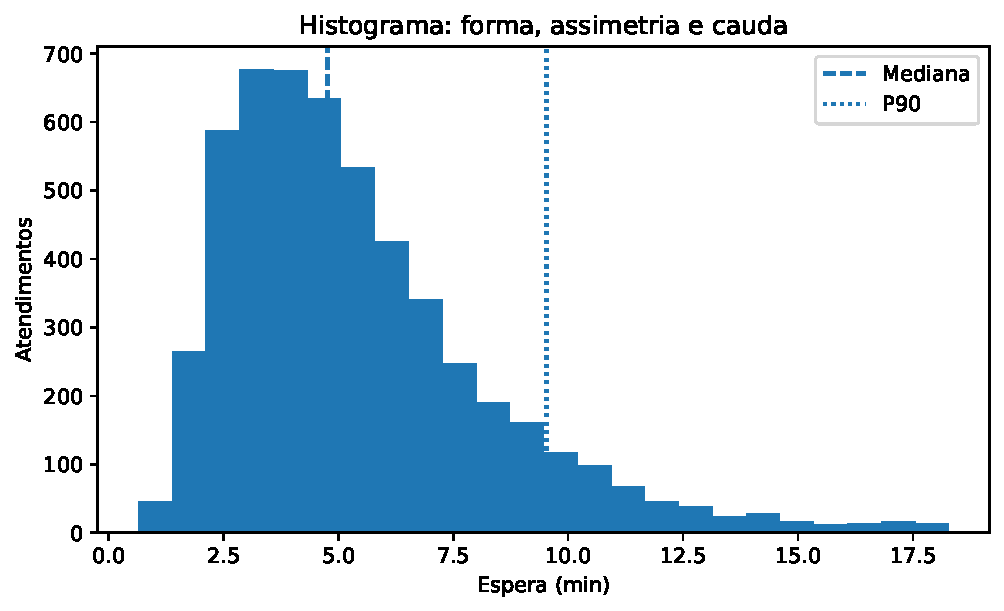
\includegraphics[width=\linewidth]{fig_06_06_histograma.pdf}
\caption*{(a) Histograma: forma e cauda.}
\end{minipage}\hfill
\begin{minipage}[t]{0.48\textwidth}
\centering
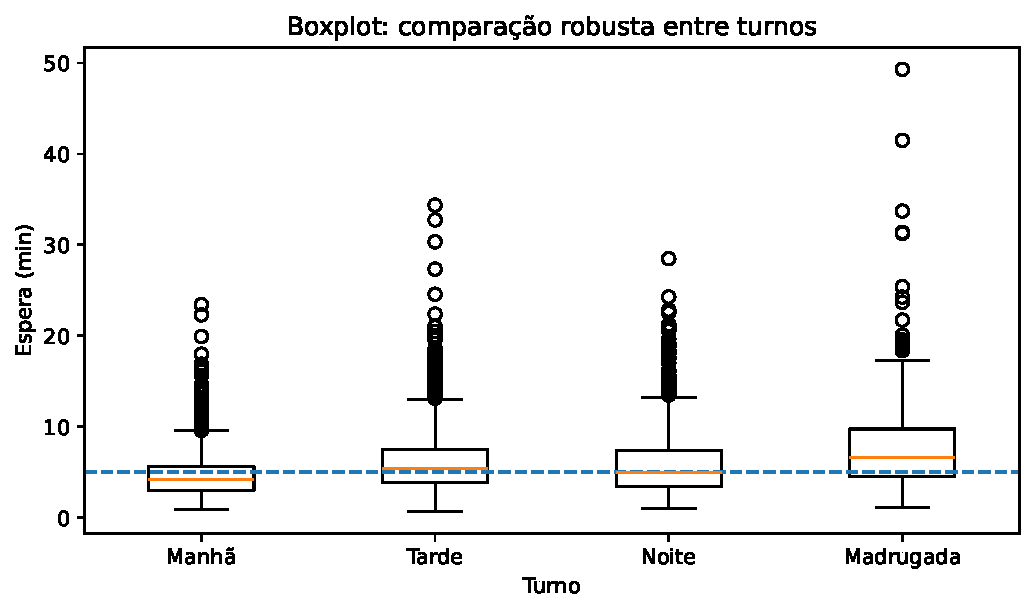
\includegraphics[width=\linewidth]{fig_06_07_boxplot.pdf}
\caption*{(b) Boxplot: comparação robusta entre grupos.}
\end{minipage}
\caption{Duas leituras da distribuição. Use histograma para perguntar ``como os valores se distribuem?'' e boxplot para perguntar ``como as distribuições dos grupos diferem em centro, dispersão e extremos?''. \FonteDidatica}
\label{fig:histograma-espera}
\label{fig:boxplot-turnos}
\end{figure}

No histograma, a largura das classes é uma decisão de visualização e de análise. Por isso, a regra de Freedman--Diaconis apresentada no texto é ponto de partida, não autorização para deixar a ferramenta decidir sem inspeção. Uma boa prática é gerar pelo menos duas larguras plausíveis e verificar se assimetria, multimodalidade e cauda permanecem. Se uma descoberta desaparece com mudança mínima de bins, ela é frágil e merece cautela. Em amostras pequenas, pontos individuais ou dotplots podem ser mais transparentes do que barras de frequência.

No boxplot, ensine os alunos a localizar Q1, mediana, Q3, IQR, hastes e pontos sinalizados, retomando o Capítulo 2. Depois peça que comparem o desenho com o histograma. A mediana pode ser parecida em dois grupos enquanto uma cauda é muito mais longa. Esse é o momento de reforçar a distinção entre resumo e distribuição completa. Violin plots e densidades podem enriquecer a leitura, mas exigem compreender suavização; não devem ser introduzidos como ornamento que ``parece mais estatístico''.

\begin{GuidedBox}
\textbf{Escolha rápida para distribuição.} Uma variável numérica, um grupo: histograma ou pontos. Muitos grupos: boxplot ou pontos resumidos. Forma detalhada importa: histograma/densidade. Comparação rápida de mediana e IQR importa: boxplot. Amostra pequena: prefira mostrar os pontos. Em qualquer opção, mantenha a mesma escala entre grupos e informe $n$ quando diferenças de tamanho da amostra puderem mudar a interpretação.
\end{GuidedBox}


\section{Relação: padrões, grupos e o limite da causalidade}

O diagrama de dispersão coloca cada unidade como ponto e codifica duas variáveis por posição. Para a central, volume diário no eixo horizontal e espera mediana no vertical podem revelar associação: dias mais cheios tendem a esperar mais. Antes de calcular uma correlação, o gráfico permite observar forma, intensidade, grupos, lacunas e valores influentes. Uma reta resumida sem pontos esconde justamente as condições sob as quais o resumo falha.

O mesmo coeficiente pode acompanhar formas muito diferentes. Uma nuvem linear, uma curva, grupos separados e um conjunto dominado por um outlier podem produzir estatísticas semelhantes. Portanto, correlação é resumo de uma relação, não substituto da visualização. Se a forma é curva, transformar a variável ou usar outro modelo pode ser adequado. Se há grupos, a associação agregada pode inverter dentro de cada grupo, fenômeno conhecido como paradoxo de Simpson.

Imagine que nos dias úteis cada turno tenha relação fraca entre volume e espera, mas fins de semana combinem baixo volume com equipe ainda menor. Ao misturar os regimes, surge forte inclinação. Colorir pontos por tipo de dia e usar painéis separados mostra a variável de contexto. Cor não deve apenas adornar: ela precisa representar uma hipótese analítica. Se nenhuma decisão depende do grupo, uma única cor reduz carga cognitiva.

Tamanho como terceiro canal exige cuidado porque o leitor percebe área. Bolhas grandes também cobrem pontos pequenos e introduzem ordem de desenho. Para uma terceira variável quantitativa, pequenos múltiplos ou cor sequencial podem ser mais legíveis; para poucas categorias, forma ou contorno pode ajudar. Um gráfico não precisa codificar todo campo disponível. Seleção é parte da clareza, e detalhes podem permanecer em tabela ou interação sob demanda.

Sobreposição aparece quando milhares de pontos ocupam posições semelhantes. Transparência, amostragem documentada, jitter para categorias, hexágonos agregados ou mapas de densidade tornam concentração visível. Cada solução muda a unidade de leitura. Um hexbin deixa de mostrar indivíduos e passa a mostrar contagens por célula. Isso deve ser informado, sobretudo quando casos raros importam. Um painel agregado pode ser acompanhado por lista auditável dos eventos extremos.

Associação visual não demonstra mecanismo causal. Uma seta, uma linha ou uma anotação não cria causalidade. A pergunta ``aumentar a equipe reduzirá a espera?'' requer considerar demanda, escala, complexidade e desenho da intervenção. O gráfico sustenta hipóteses e identifica padrões que merecem teste. O título responsável diz ``maior volume coincide com maior espera'', não ``volume causa atraso'', a menos que a evidência tenha identificado esse efeito.



A Figura~\ref{fig:scatter-volume} materializa a ideia principal do diagrama de dispersão: cada observação possui uma posição em $X$ e outra em $Y$. O leitor procura direção, forma, força, grupos e pontos influentes. A linha tracejada é apenas um resumo linear global; ela não deve ser apresentada sem os pontos. A separação entre dias úteis e fins de semana mostra que uma terceira variável pode alterar o padrão observado.

\begin{figure}[H]
\centering
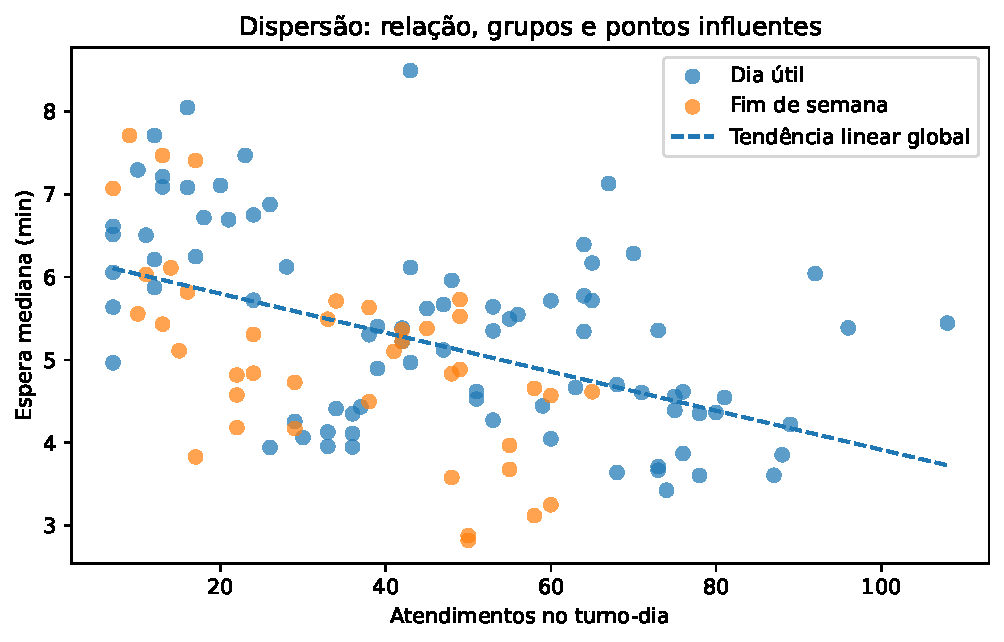
\includegraphics[width=0.78\textwidth]{fig_06_08_dispersao.pdf}
\caption{Dispersão entre volume e espera, distinguindo tipos de dia. Antes de calcular correlação, observe forma, grupos e valores influentes. \FonteDidatica}
\label{fig:scatter-volume}
\end{figure}

Um exemplo clássico ajuda a impedir que o aluno substitua gráfico por coeficiente. O quarteto de Anscombe reúne quatro conjuntos com estatísticas-resumo muito semelhantes, incluindo médias, variâncias, correlação e reta de regressão, mas com estruturas visuais radicalmente diferentes \cite{anscombe1973}. As quatro miniaturas da Figura~\ref{fig:anscombe} devem ser mostradas antes de revelar essa propriedade. Peça à turma que descreva o que cada conjunto exigiria como diagnóstico.

\begin{figure}[H]
\centering
\begin{minipage}[t]{0.235\textwidth}\centering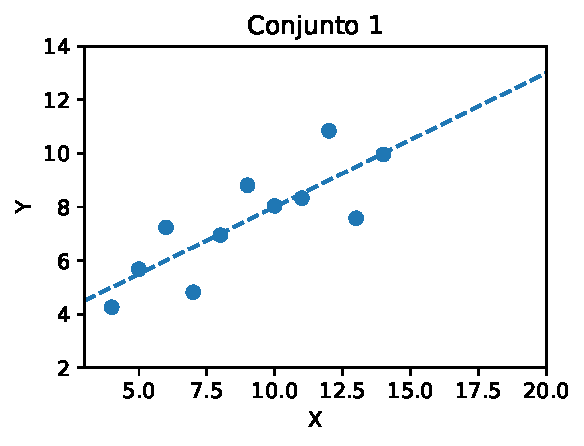
\includegraphics[width=\linewidth]{fig_06_08_anscombe_1.pdf}\end{minipage}\hfill
\begin{minipage}[t]{0.235\textwidth}\centering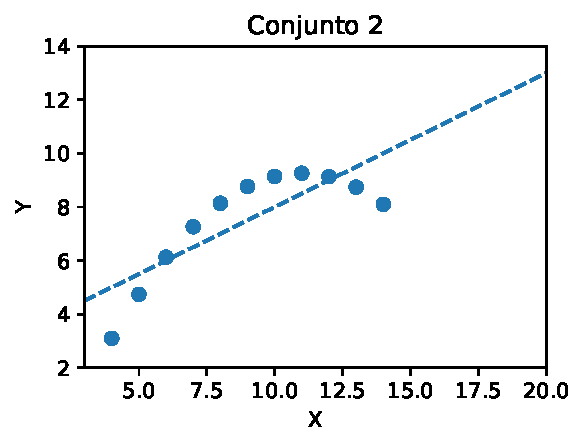
\includegraphics[width=\linewidth]{fig_06_08_anscombe_2.pdf}\end{minipage}\hfill
\begin{minipage}[t]{0.235\textwidth}\centering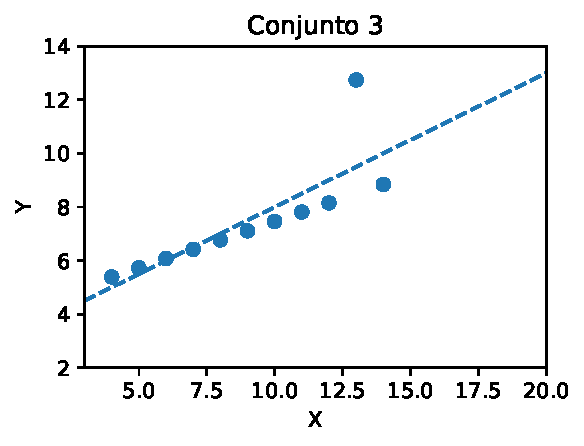
\includegraphics[width=\linewidth]{fig_06_08_anscombe_3.pdf}\end{minipage}\hfill
\begin{minipage}[t]{0.235\textwidth}\centering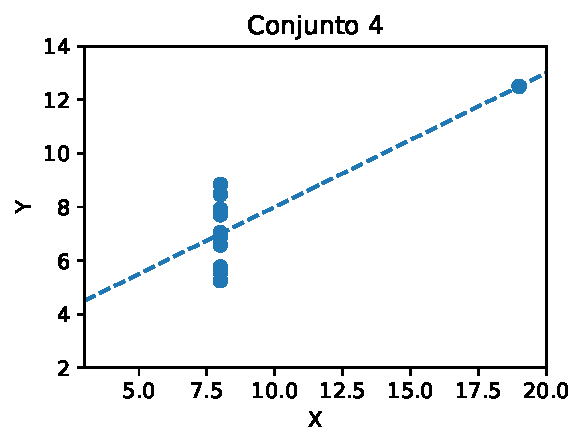
\includegraphics[width=\linewidth]{fig_06_08_anscombe_4.pdf}\end{minipage}
\caption{Quarteto de Anscombe: estatísticas-resumo semelhantes não implicam a mesma forma. Reproduzido numericamente a partir do exemplo clássico de Anscombe \cite{anscombe1973}.}
\label{fig:anscombe}
\end{figure}

A escolha do scatterplot é forte quando ambas as variáveis são quantitativas e cada ponto representa uma unidade comparável. Se uma variável é categórica, barras, boxplots ou pontos com jitter podem ser mais adequados. Se há milhões de observações, transparência e agregação espacial podem revelar densidade. Se a relação tem tempo, às vezes uma trajetória ou facetas é melhor. Não transforme scatter em matriz multicolorida apenas porque existem outras colunas disponíveis: cada canal adicional deve corresponder a uma hipótese de leitura.

\begin{GuidedBox}
\textbf{Pergunta para a turma.} Se $r=0{,}8$, qual gráfico devemos imaginar? Nenhum em particular. O coeficiente resume associação linear sob certas condições, mas não informa sozinho se há curva, dois grupos, um ponto dominante ou mudança de regime. A ordem responsável é: visualize $\rightarrow$ descreva a forma $\rightarrow$ investigue contexto $\rightarrow$ então use correlação ou regressão como resumo apropriado.
\end{GuidedBox}


\section{Composição: partes, totais e denominadores}

Composição pergunta como um total se divide. Uma barra empilhada mostra parte e todo quando as categorias são mutuamente exclusivas e o denominador é explícito. Para um único mês, uma barra de 100\% permite ler participação dos canais; para valores absolutos, a altura total também comunica volume. Misturar os dois objetivos na mesma escala confunde. Se a decisão é capacidade, volume absoluto importa; se é mudança de mix, proporção pode ser o foco.

Somente os segmentos junto à mesma base são comparados com precisão. Em barras empilhadas, o primeiro segmento parte de zero; os internos flutuam. Por isso, acompanhar a participação de quatro canais ao longo de doze meses pode ser melhor com linhas de participação ou pequenos múltiplos. O empilhamento é útil para uma visão compacta do todo, mas não transforma todas as partes em comparações igualmente fáceis.

Gráficos de setores codificam proporção por ângulo e área. Podem comunicar poucas partes muito diferentes, desde que somem 100\% e não haja valores negativos. Tornam-se fracos quando há muitas fatias, diferenças pequenas ou necessidade de comparar períodos. Uma barra ordenada costuma permitir julgamento mais preciso. Donut remove a região central, reduzindo a referência angular, embora abra espaço para um rótulo; o espaço ganho não corrige a dificuldade perceptiva.

Treemaps usam área e acomodam hierarquias, mas são inadequados para diferenças sutis. Um retângulo duas vezes maior representa o dobro, porém formatos e posições variados dificultam a estimativa. Sunbursts acrescentam anéis e ângulos, aumentando a carga. Essas formas são úteis para exploração de estrutura quando espaço é limitado, não como escolha universal. Para mostrar receita por canal e produto com comparação precisa, dois painéis de barras ou uma tabela hierárquica podem ser melhores.

O denominador pode mudar no tempo. Se a participação do chat cresce de 20\% para 30\%, isso pode ocorrer com chat estável e queda dos demais canais. Mostre também o total ou declare a mudança absoluta. Decomposições devem fechar: soma das partes igual ao todo, categorias sem sobreposição e tratamento visível de ``outros'' e ausentes. Uma categoria ``outros'' que passa de 5\% para 35\% destrói a interpretabilidade e pede revisão da classificação.

Composição acumulada também aparece em curvas de Pareto. Ordenam-se categorias pela contribuição, calculando $p_k=\sum_{i=1}^{k}x_i/\sum_i x_i$, e observa-se quanto do total está concentrado nas primeiras posições. Se três motivos respondem por 72\% das reclamações, isso orienta investigação, mas não prova que tratá-los produzirá 72\% de redução: causas podem se sobrepor e custos diferem. A curva deve manter barras de valores e linha acumulada com unidades claramente separadas; uma tabela curta pode evitar o eixo duplo.

Waterfall e áreas empilhadas respondem perguntas específicas. O primeiro decompõe como acréscimos e reduções levam de um saldo inicial a outro; o segundo enfatiza evolução do total e composição contínua. Ambos dependem de ordem e base corretas. Nunca use área empilhada para séries que podem ser negativas sem tratamento explícito, pois a linha de base se torna ambígua. Em composição, a pergunta central é sempre ``parte de qual total, em qual momento e sob quais regras?''.



A Figura~\ref{fig:composicao-pizza}, nos painéis (a) e (b), usa exatamente as mesmas participações por canal. O setor é reconhecível e pode funcionar quando existem poucas partes muito diferentes e a mensagem principal é ``parte de um todo''. Porém, quando o leitor precisa comparar diferenças, as barras colocam todas as magnitudes sobre uma escala comum e reduzem a necessidade de estimar ângulos e áreas. Estudos de percepção gráfica sustentam a preferência por canais de posição e comprimento em tarefas quantitativas precisas \cite{cleveland1984,heer2010,zeng2023}.

\begin{figure}[H]
\centering
\begin{minipage}[t]{0.44\textwidth}
\centering
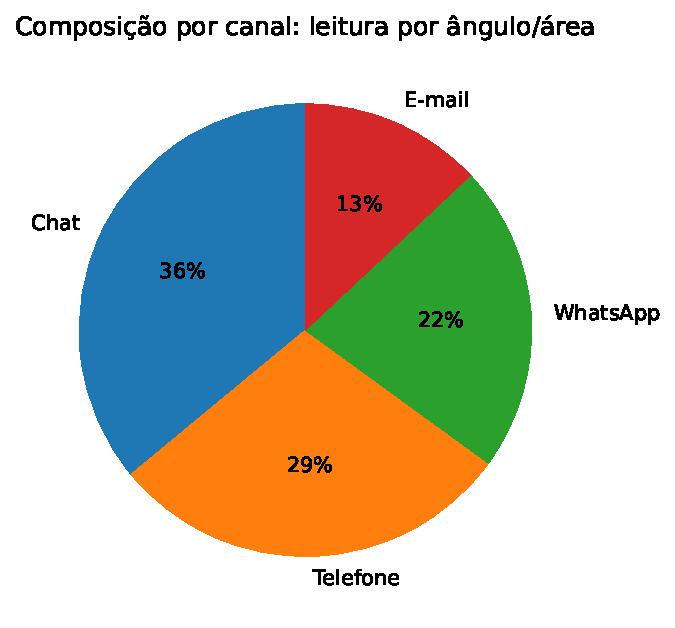
\includegraphics[width=\linewidth]{fig_06_09a_pizza.pdf}
\caption*{(a) Setor: comunicação de composição simples.}
\end{minipage}\hfill
\begin{minipage}[t]{0.52\textwidth}
\centering
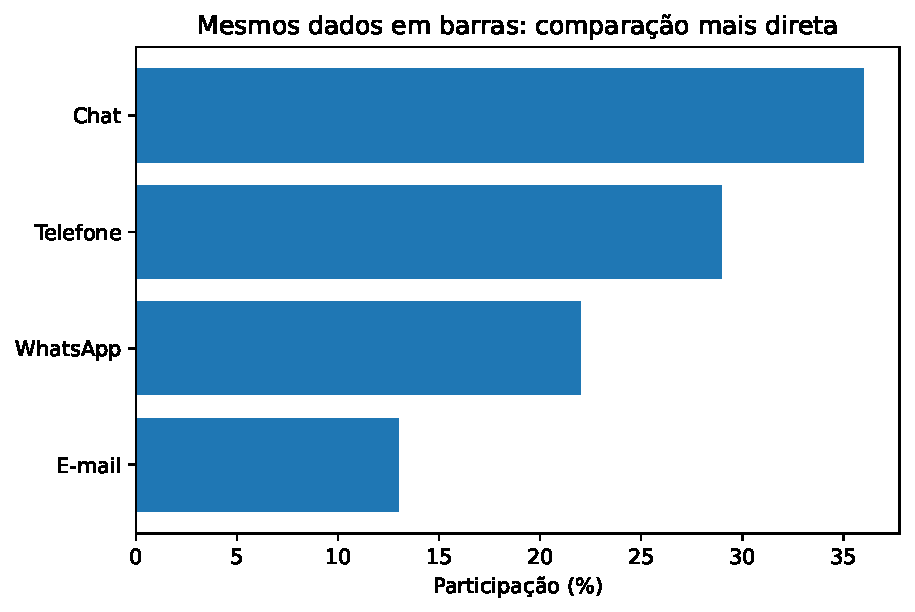
\includegraphics[width=\linewidth]{fig_06_09b_barras_composicao.pdf}
\caption*{(b) Barras: diferenças ficam mais fáceis de comparar.}
\end{minipage}
\caption{Mesmos dados de composição, tarefas perceptivas diferentes. \FonteDidatica}
\label{fig:composicao-pizza}
\label{fig:composicao-barras}
\end{figure}

Área empilhada é adequada quando se deseja acompanhar simultaneamente a evolução do total e a composição ao longo do tempo. A Figura~\ref{fig:area-empilhada} mostra crescimento do volume enquanto o mix migra de telefone para canais digitais. O limite é perceptivo: somente a primeira faixa possui uma base estável; comparar exatamente as faixas internas é difícil. Se a pergunta muda para ``qual canal cresceu mais?'', linhas separadas ou pequenos múltiplos provavelmente são superiores.

\begin{figure}[H]
\centering
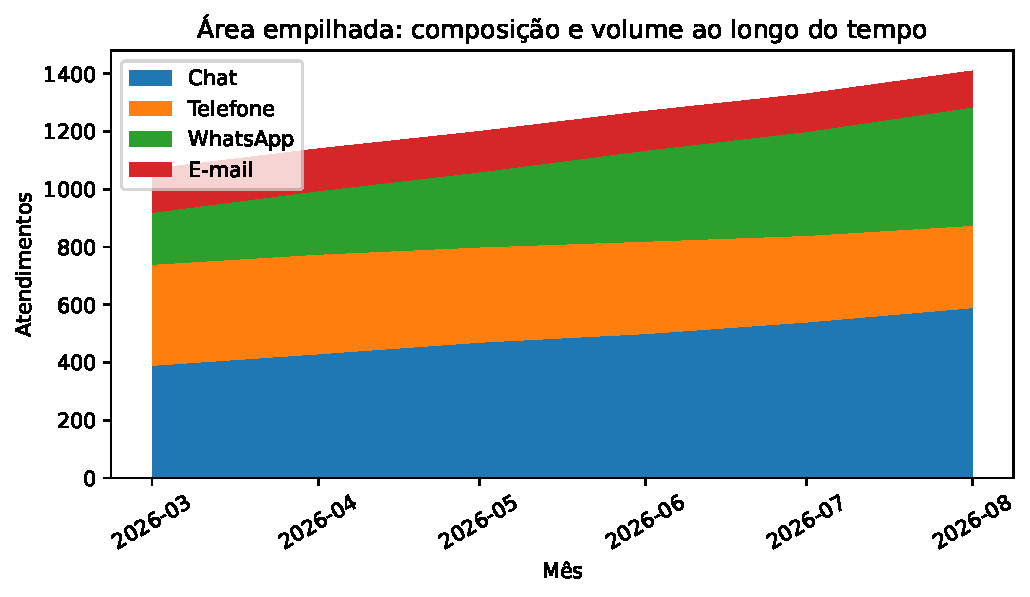
\includegraphics[width=0.82\textwidth]{fig_06_10_area_empilhada.pdf}
\caption{Área empilhada: útil para evolução do total e composição, menos adequada para comparação precisa entre séries internas. \FonteDidatica}
\label{fig:area-empilhada}
\end{figure}

A curva de Pareto também combina duas leituras: contribuição individual e contribuição acumulada. Para evitar um eixo duplo confuso, a Figura~\ref{fig:pareto} expressa ambos em percentuais. As barras identificam os motivos mais frequentes; a linha mostra quanto do total já foi explicado pelas primeiras categorias. O princípio ``80/20'' não é uma lei que precisa aparecer nos dados. A linha de 80\% é apenas referência operacional para perguntar quanto da massa está concentrada.

\begin{figure}[H]
\centering
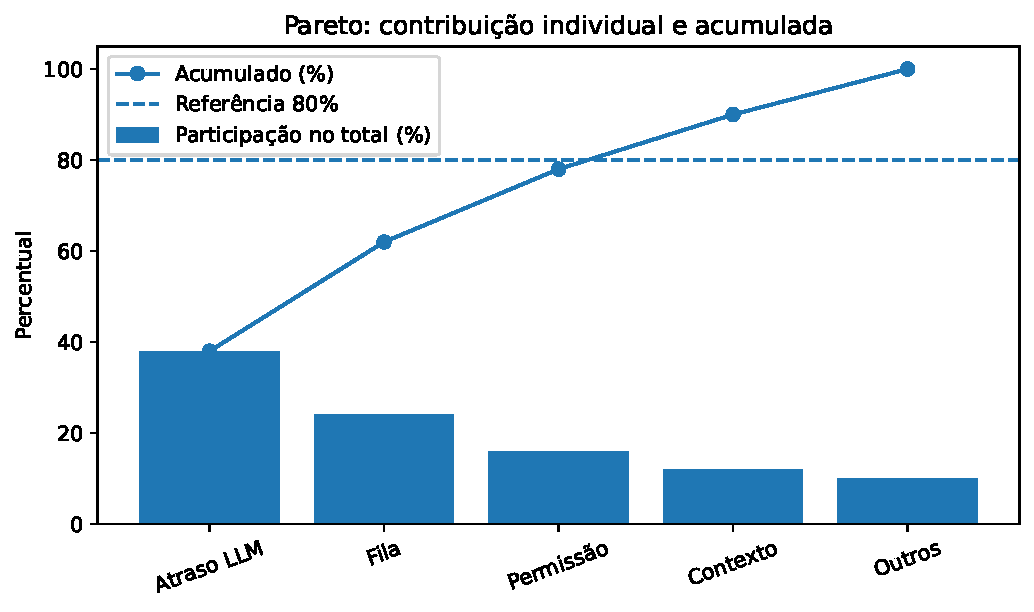
\includegraphics[width=0.80\textwidth]{fig_06_10_pareto.pdf}
\caption{Pareto com barras de participação e acumulado na mesma unidade percentual. \FonteDidatica}
\label{fig:pareto}
\end{figure}

\begin{GuidedBox}
\textbf{Escolha rápida para composição.} Poucas partes e mensagem grosseira de ``parte do todo'': setor pode funcionar. Comparação precisa: barras. Mix ao longo do tempo com total relevante: área ou barra empilhada. Participação ao longo do tempo com comparação entre partes: linhas ou pequenos múltiplos. Hierarquia: treemap pode ajudar a explorar estrutura, mas não é primeira escolha para diferenças sutis.
\end{GuidedBox}


\section{Escalas, eixos e normalização}

Escala é a regra que converte valores em posições, comprimentos ou cores. Em escala linear, diferenças iguais ocupam distâncias iguais: a distância de 2 para 4 é igual à de 8 para 10. Em escala logarítmica, razões iguais ocupam distâncias iguais: 1, 10, 100 e 1.000 ficam igualmente espaçados. A transformação é útil para ordens de grandeza e crescimento multiplicativo, mas valores zero e negativos exigem tratamento e a leitura precisa ser declarada.

Um eixo deve mostrar unidade, limites, marcas e transformação. Abreviar ``mil'' e ``milhão'' sem consistência pode produzir erros de mil vezes. Datas devem respeitar intervalos reais. Eixos invertidos só fazem sentido quando a convenção do domínio os torna naturais, como posição em ranking ou profundidade. Grades leves ajudam a estimar; grades escuras competem com os dados. Rótulos de todos os pontos criam uma tabela mal diagramada.

Dois eixos verticais permitem sobrepor séries de unidades diferentes, porém qualquer inclinação aparente pode ser fabricada escolhendo limites independentes. Receita e satisfação podem parecer mover-se juntas em uma configuração e divergir em outra. Alternativas incluem painéis alinhados, índice com base comum ou normalização explicitamente justificada. Se o eixo duplo for indispensável, cores devem vincular série e eixo, limites devem ser documentados e a interpretação não deve apoiar-se apenas no paralelismo visual.

Normalizar responde a perguntas comparativas. Dividir por população produz taxa per capita; dividir pelo primeiro período produz índice; subtrair a média e dividir pelo desvio-padrão produz escore $z=(x-\bar{x})/s$. Se um turno tem espera 7, média histórica 5 e desvio 1, seu $z=2$: está dois desvios acima da média daquele turno. Isso permite comparar desvios relativos entre operações, mas remove minutos e pressupõe que média e desvio sejam referências úteis.

Min--max, $x'=(x-\min)/(\max-\min)$, coloca valores entre zero e um. Um novo extremo muda todos os valores transformados, e a escala não informa distância substantiva. Percentual de meta, por sua vez, depende da direção do indicador: 120\% da meta pode ser bom para vendas e ruim para espera. Toda normalização precisa de semântica, fórmula e referência. ``Pontuação normalizada'' sem esses elementos é uma caixa-preta visual.

Uma boa auditoria refaz a leitura em unidades originais. Se um painel usa índices para comparar tendências, disponibilize valores absolutos em tooltip, tabela ou painel adjacente. Se usa log, mostre marcas como 1, 10 e 100, não expoentes opacos. Se corta o eixo, sinalize e explique. Escalas não são rodapés técnicos: elas definem o que distância significa e, portanto, participam da afirmação principal.



As Figuras~\ref{fig:escala-linear} e~\ref{fig:escala-log} mostram por que uma transformação de escala altera a pergunta perceptiva. Na escala linear, distâncias iguais significam diferenças iguais. Na logarítmica, distâncias iguais significam razões iguais. A mesma série de custos com ordens de grandeza diferentes fica ``achatada'' perto de zero na escala linear; o log distribui melhor os valores, porém muda o significado de distância. O leitor precisa ser avisado, e valores zero ou negativos exigem solução coerente com o domínio.

\begin{figure}[H]
\centering
\begin{minipage}[t]{0.48\textwidth}
\centering
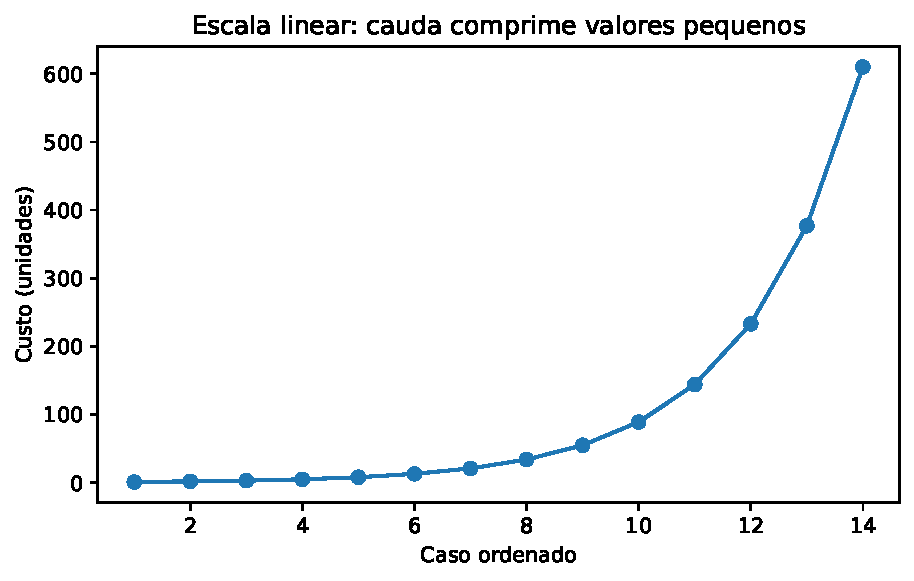
\includegraphics[width=\linewidth]{fig_06_11a_linear.pdf}
\caption*{(a) Escala linear.}
\end{minipage}\hfill
\begin{minipage}[t]{0.48\textwidth}
\centering
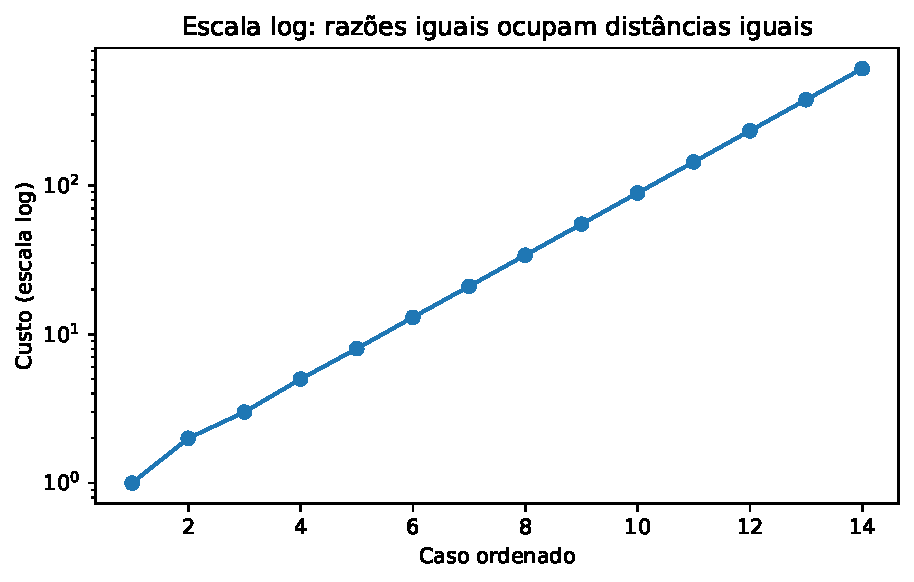
\includegraphics[width=\linewidth]{fig_06_11b_log.pdf}
\caption*{(b) Escala logarítmica.}
\end{minipage}
\caption{Escala não é acabamento: ela define o significado da distância visual. \FonteDidatica}
\label{fig:escala-linear}
\label{fig:escala-log}
\end{figure}

Uma forma prática de ensinar normalização é perguntar o que deve permanecer comparável. Se queremos comparar crescimento relativo de receita e usuários, indexar ambos em 100 numa data-base torna ritmos comparáveis, mas esconde níveis originais. Se queremos comparar taxa de reclamação entre regiões de população diferente, dividir por denominador adequado preserva risco relativo. Se queremos comparar desvios em escalas distintas, o escore $z$ pode ser útil. Em todos os casos, normalização cria uma nova variável; ela precisa de nome, fórmula e interpretação próprios.

O eixo duplo merece uma regra conservadora. Se duas séries possuem unidades diferentes, tente primeiro dois painéis alinhados, uma transformação comum justificada ou uma tabela complementar. Dois eixos independentes permitem fabricar paralelismo por escolha de limites. Mesmo quando a intenção é honesta, o leitor pode interpretar inclinações como equivalentes. A prática de visualização orientada à decisão prefere comparações cuja semântica seja estável e auditável \cite{few2012,cairo2016,wilke2019}.

\begin{GuidedBox}
\textbf{Checklist de escala.} Unidade aparece? zero é necessário para a marca usada? há corte de eixo? a transformação é linear, log, índice, taxa, percentual ou $z$? o leitor consegue voltar à unidade original? filtros podem mudar mínimo, máximo ou denominador? Se uma dessas respostas estiver escondida, a distância no gráfico pode significar outra coisa do que o leitor imagina.
\end{GuidedBox}


\section{Cor, contraste e acessibilidade}

Cor pode distinguir categorias, ordenar intensidade ou separar desvios. Como cor é um canal perceptivo com propriedades próprias de luminância, matiz e contraste, seu uso precisa acompanhar o tipo de variável e a tarefa do leitor \cite{ware2021,wilke2019}. Paletas qualitativas usam matizes distintos sem ordem para poucas categorias. Paletas sequenciais variam luminosidade para valores do menor ao maior. Paletas divergentes partem de um centro substantivo, como zero ou meta, e usam duas direções. Aplicar arco-íris a uma taxa cria fronteiras artificiais e não oferece ordem perceptiva estável. A paleta deve nascer do tipo de variável.

O destaque funciona por contraste, não por quantidade de pigmento. Se todas as barras têm cor intensa, nenhuma se destaca. Na central, barras cinza com a madrugada em laranja guiam o olhar para a exceção; a cor precisa ser acompanhada por título ou anotação que explique por quê. Usar vermelho e verde como únicos portadores de ``ruim'' e ``bom'' exclui parte dos leitores e falha em impressão. Forma, posição, rótulo ou padrão devem fornecer redundância.

Luminosidade costuma comunicar ordem melhor que mudança arbitrária de matiz. Em um mapa de calor, células mais escuras podem representar maior espera, com legenda contínua e limites. Se os valores cruzam uma meta, uma escala divergente centrada em cinco minutos torna o desvio explícito. Centrar automaticamente na média dos dados mudaria o significado a cada filtro. O centro deve vir do domínio, não da conveniência gráfica.

Contraste de texto, tamanho de fonte e espaço em branco também são acessibilidade. Legendas distantes exigem memória; rotular linhas diretamente reduz busca. Siglas devem ser definidas. Texto alternativo deve registrar mensagem, eixos, período, padrão e exceções, não apenas dizer ``gráfico de linhas''. Uma tabela acessível pode acompanhar a figura quando valores exatos importam. A experiência não termina na tela colorida do autor.

Cor geográfica merece cautela. Em mapas coropléticos, área grande chama atenção mesmo com taxa moderada; contagens favorecem regiões populosas. Taxas normalizadas são normalmente mais informativas, desde que populações pequenas e incerteza sejam sinalizadas. Para localização de eventos, pontos podem ser adequados; para densidade, agregação espacial evita sobreposição. Um mapa só deve ser escolhido quando geografia participa da pergunta, não porque há uma coluna de estado.

Teste a figura em escala de cinza, projeção, celular e impressão. Verifique se a conclusão continua possível sem depender de hover. Paletas perceptualmente uniformes disponíveis em bibliotecas modernas ajudam, mas não dispensam julgamento. A ferramenta pode sugerir cores; o analista valida contraste, semântica, consistência e consequências. Estética apoia confiança quando torna estrutura legível, não quando mascara fragilidade.



O heatmap da Figura~\ref{fig:heatmap} mostra um uso apropriado de cor: a posição identifica dia e hora, enquanto a intensidade da célula codifica espera. A tarefa não é recuperar 5,37 minutos com precisão; é localizar regiões de concentração. Esse tipo de gráfico funciona especialmente bem para matrizes como hora $\times$ dia, produto $\times$ região ou variável $\times$ variável. Se o valor exato é a tarefa principal, tabela ou rótulo sob demanda pode ser superior.

\begin{figure}[H]
\centering
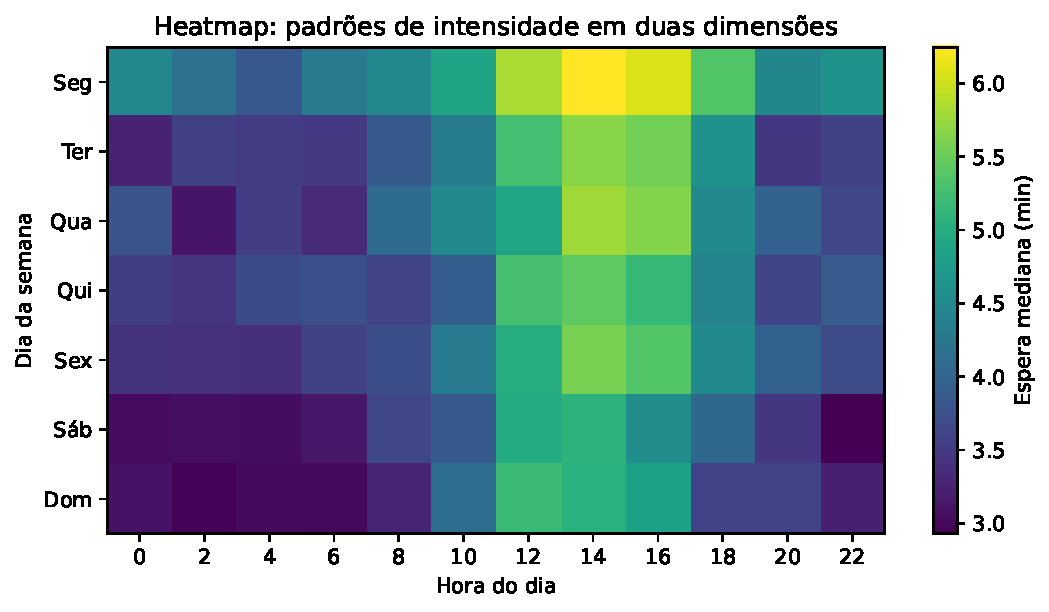
\includegraphics[width=0.84\textwidth]{fig_06_12_heatmap.pdf}
\caption{Heatmap: cor resume intensidade em uma matriz e ajuda a localizar padrões espaciais ou temporais. \FonteDidatica}
\label{fig:heatmap}
\end{figure}

Ensine três famílias de paleta pela semântica. \textbf{Qualitativa}: categorias sem ordem, usando cores distintas e poucas classes. \textbf{Sequencial}: números do baixo ao alto, normalmente com luminosidade ordenada. \textbf{Divergente}: desvios em torno de um centro substantivo, como zero, meta ou referência. Esse centro precisa vir do problema. A percepção de cor depende de contraste, contexto e capacidades visuais, razão pela qual a literatura de percepção recomenda cuidado especial com saturação, luminosidade e mapas de cor \cite{ware2021,wilke2019}.

O mapa coroplético é um caso especializado de cor. Ele deve entrar somente quando a geografia participa da pergunta. Pintar estados por número absoluto de chamados costuma destacar regiões populosas; pintar por taxa pode ser mais justo, mas regiões com denominadores pequenos ficam instáveis. Portanto, mapa exige legenda, unidade, denominador e, quando relevante, tamanho da amostra. ``Tenho uma coluna de estado'' não é justificativa suficiente para um mapa.

\begin{GuidedBox}
\textbf{Teste de acessibilidade.} Imprima em escala de cinza ou reduza a saturação: a ordem e o destaque continuam visíveis? O gráfico depende apenas de vermelho contra verde? O título e os rótulos explicam a exceção sem exigir legenda distante? Há alternativa textual ou tabela quando valores exatos importam? A cor deve reduzir esforço, não ser o único portador da mensagem.
\end{GuidedBox}


\section{Múltiplos painéis, facetas e comparações justas}

Pequenos múltiplos repetem a mesma gramática para grupos ou métricas. Quatro painéis de linha, um por turno, permitem enxergar sazonalidade sem sobreposição. A repetição reduz aprendizado porque o leitor entende um painel e transfere a regra. Para comparação justa, eixos devem compartilhar limites quando o nível importa. Escalas livres podem revelar forma interna, mas fazem séries de amplitudes distintas parecer igualmente variáveis.

Um painel geral e outro de detalhe podem coexistir. O primeiro mostra a série anual; o segundo amplia os últimos trinta dias. A relação precisa ser explícita por título, faixa destacada ou anotação. Sem isso, o detalhe parece outra população. Zoom é útil para investigar, mas não pode apagar a posição do recorte no todo. Contexto e foco são duas vistas da mesma evidência.

Facetar por uma variável relevante ajuda a detectar heterogeneidade. Se a queda de espera existe apenas na manhã, uma linha agregada pode atribuí-la à central inteira. Facetas por turno revelam a diferença; facetas por dezenas de agentes produzem miniaturas ilegíveis. A quantidade de painéis deve seguir a decisão. Para muitos grupos, ordenar por uma métrica, destacar exceções e oferecer exploração filtrável é mais eficiente.

Dashboards combinam gráficos, mas proximidade sugere relação. Colocar uma linha de receita ao lado de reclamações pode convidar inferência causal mesmo sem conexão. Títulos e organização precisam dizer se os painéis compartilham filtros, período e população. Um filtro silencioso é especialmente perigoso: o total no topo pode permanecer global enquanto a tabela abaixo mostra apenas um turno. Indicadores de estado e subtítulos dinâmicos tornam o contexto auditável.

A hierarquia visual distribui atenção. No topo, a pergunta e poucos indicadores; no centro, evidência principal; abaixo, diagnóstico e detalhe. Essa organização não é regra rígida, mas consequência do percurso decisório. Uma grade coerente, alinhamento e espaço reduzem busca. Repetir vinte cartões de KPI concede igual peso a sinais desiguais e transforma o dashboard em inventário. O que não sustenta a decisão pode sair ou ficar sob demanda.

Interação adiciona possibilidades e riscos. Filtro, seleção e tooltip permitem detalhe; também podem esconder o estado que produziu a figura. Exporte o contexto com o gráfico, mantenha valores padrão seguros e ofereça caminho de retorno. Uma captura de tela deve conservar data, filtros e fonte. O painel é uma interface para argumentos de dados, e sua reprodutibilidade depende tanto das consultas quanto dos estados de interação.



Os quatro gráficos da Figura~\ref{fig:small-multiples} usam exatamente a mesma escala vertical e o mesmo intervalo de datas. Essa repetição transforma cada painel em uma unidade comparável. O leitor aprende a gramática uma vez e passa a procurar diferenças de forma, nível e ruptura. É uma solução superior a sobrepor quatro linhas quando as séries se cruzam muito ou quando a identificação por cor exige esforço contínuo.

\begin{figure}[H]
\centering
\begin{minipage}[t]{0.48\textwidth}\centering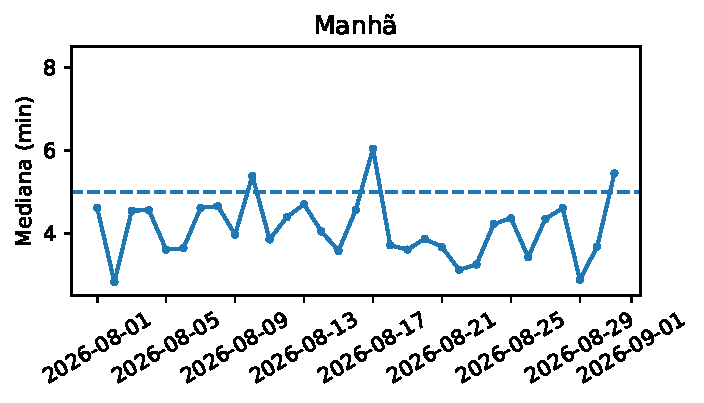
\includegraphics[width=\linewidth]{fig_06_13_manha.pdf}\end{minipage}\hfill
\begin{minipage}[t]{0.48\textwidth}\centering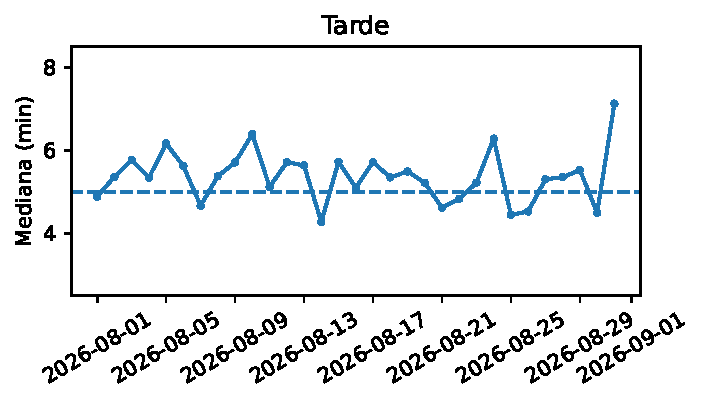
\includegraphics[width=\linewidth]{fig_06_13_tarde.pdf}\end{minipage}\\[0.4em]
\begin{minipage}[t]{0.48\textwidth}\centering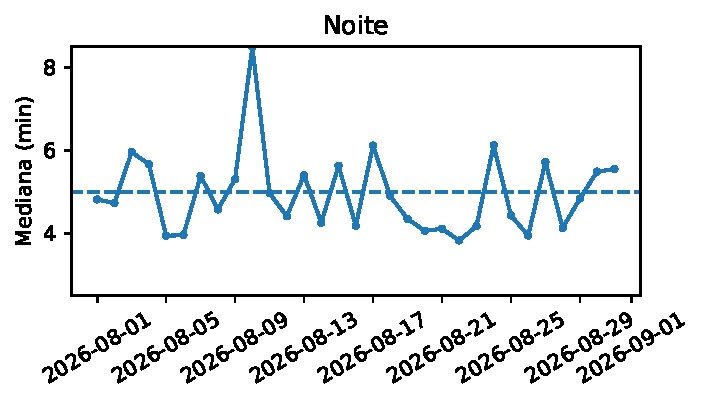
\includegraphics[width=\linewidth]{fig_06_13_noite.pdf}\end{minipage}\hfill
\begin{minipage}[t]{0.48\textwidth}\centering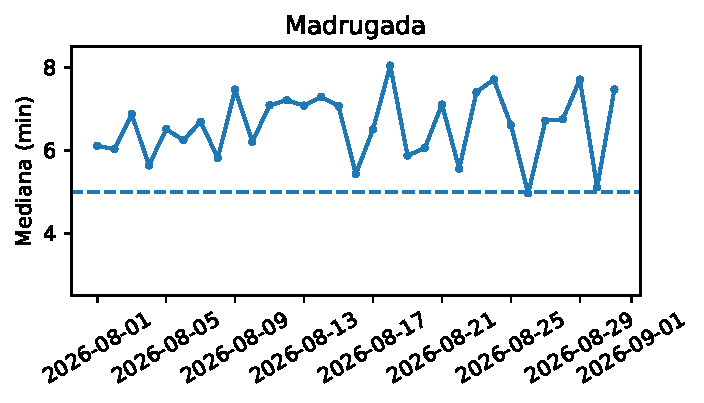
\includegraphics[width=\linewidth]{fig_06_13_madrugada.pdf}\end{minipage}
\caption{Pequenos múltiplos por turno. Escalas comuns permitem comparação justa de nível e variabilidade. \FonteDidatica}
\label{fig:small-multiples}
\end{figure}

Facetas são especialmente valiosas quando a agregação geral esconde heterogeneidade. Se a média da central melhora apenas porque aumentou a participação da manhã, o painel agregado pode sugerir melhoria operacional em todos os turnos. Separar por turno permite verificar se o padrão é compartilhado. Essa ideia se conecta ao capítulo anterior: agregações podem mascarar relações internas, e a visualização por grupos ajuda a investigar antes de resumir.

Escala livre entre facetas só deve ser usada quando a tarefa principal é comparar \emph{forma interna}, não magnitude. Se cada painel escolhe seu próprio mínimo e máximo, uma série que varia de 4,0 a 4,3 pode parecer tão instável quanto outra que varia de 2 a 10. Quando a magnitude importa, mantenha limites comuns. Quando a forma é a tarefa e os níveis são muito diferentes, uma escala livre pode ser útil, mas o título deve deixar essa decisão explícita.

\begin{GuidedBox}
\textbf{Pergunta para a turma.} Por que não colocar todos os turnos na mesma linha com quatro cores? Pode ser adequado para poucas séries bem separadas. O problema aparece quando há cruzamentos, legenda distante e muitos grupos. Facetas trocam compactação por legibilidade. A escolha depende de quanto o leitor precisa comparar séries entre si versus acompanhar cada série individualmente.
\end{GuidedBox}


\section{Incerteza: não desenhar estimativas como certezas}

Todo resumo contém incerteza de medição, amostragem, processamento ou previsão. Uma média calculada sobre todos os atendimentos registrados ainda pode omitir quedas do sistema e registros incompletos. Uma estimativa amostral acrescenta variação entre amostras. Um gráfico honesto distingue valor observado, estimativa e meta. Casas decimais em excesso não criam precisão; frequentemente apenas escondem a origem aproximada do número.

Intervalos de confiança representam procedimento de estimação, não faixa onde ``95\% dos dados estão''. Para uma média com erro-padrão $EP=s/\sqrt{n}$, uma aproximação de 95\% é $\bar{x}\pm1{,}96EP$ em condições adequadas. Se $\bar{x}=5$, $s=2$ e $n=100$, então $EP=0{,}2$ e o intervalo aproximado é $[4{,}61;5{,}39]$. O gráfico deve informar método, nível e tamanho da amostra, especialmente ao comparar grupos.

Barras de erro sobrepostas não resolvem sozinhas um teste de diferença, e ausência de sobreposição não explica relevância prática. Mostre efeito e intervalo em unidade compreensível. Uma redução estimada de 0,1 minuto com intervalo estreito pode ser estatisticamente clara e operacionalmente irrelevante; redução de 1 minuto com intervalo largo pode justificar coleta adicional. A decisão combina magnitude, incerteza, custo e reversibilidade.

Previsões precisam de faixas que normalmente se alargam com o horizonte. Uma linha pontual até dezembro sugere conhecimento que o modelo não possui. Cenários devem ser rotulados como cenários, não confundidos com intervalos probabilísticos. Se uma área sombreada representa P10--P90, explique que ela depende do modelo e dos pressupostos. Choques fora do histórico podem permanecer fora da faixa, logo incerteza quantificada não equivale a garantia.

Dados suprimidos por privacidade ou baixa contagem devem aparecer como ausência explicada, não zero. Em mapas e taxas, regiões com denominadores pequenos produzem grande volatilidade; transparência, hachura ou painel de tamanho da amostra ajudam a impedir ranking injusto. Uma taxa de 50\% baseada em dois casos não tem o mesmo peso que 48\% baseada em dois mil. Codificar apenas a taxa remove essa diferença essencial.

A incerteza também pode ser comunicada por linguagem. ``Estima-se'', ``nos registros disponíveis'' e ``o padrão é compatível com'' delimitam a afirmação; ``comprovou'' exige evidência mais forte. Não se trata de enfraquecer a mensagem, mas de calibrá-la. Um leitor que conhece limites pode decidir melhor do que outro seduzido por precisão falsa. Visualização responsável conserva dúvida relevante sem transformar toda conclusão em paralisia.



A Figura~\ref{fig:intervalos} mostra uma alternativa importante às barras de média: um ponto representa a estimativa e uma linha representa a incerteza. Como a posição do ponto é a marca principal, não precisamos preencher uma barra desde zero. O tamanho da amostra aparece no rótulo porque a mesma média baseada em centenas ou em poucos casos não tem a mesma estabilidade. O intervalo ilustrativo não transforma automaticamente uma comparação em ``significativa''; ele comunica uma faixa de estimação sob um procedimento declarado.

\begin{figure}[H]
\centering
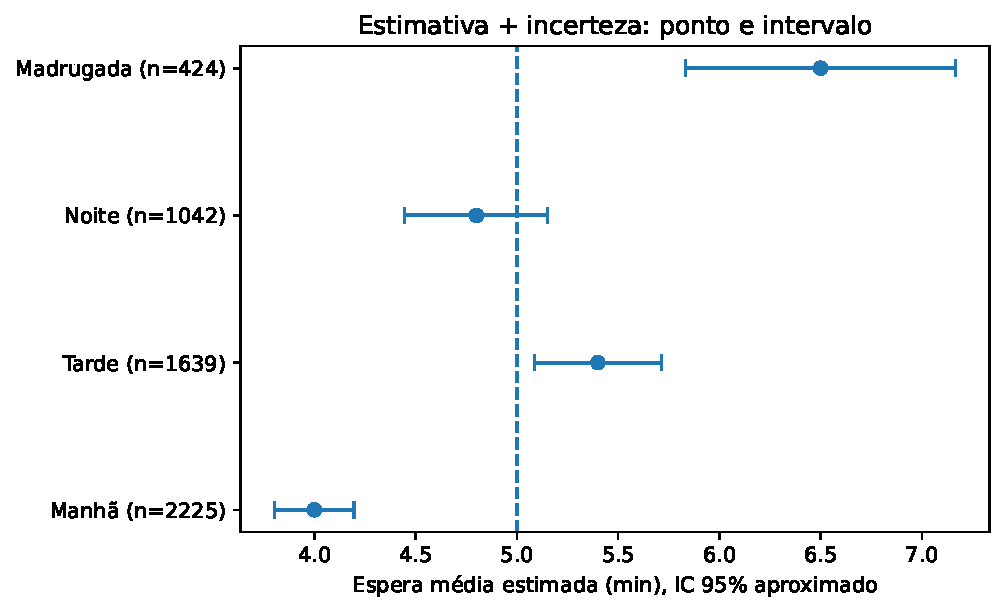
\includegraphics[width=0.82\textwidth]{fig_06_14_intervalos.pdf}
\caption{Ponto + intervalo: visualização de estimativa e incerteza, com tamanho da amostra visível. \FonteDidatica}
\label{fig:intervalos}
\end{figure}

Previsão exige outro tipo de incerteza. Na Figura~\ref{fig:previsao}, o passado é observado e o futuro é estimado. A faixa se alarga porque o horizonte aumenta e, com ele, a incerteza acumulada. Uma linha única no futuro cria a impressão de que cada ponto é conhecido com a mesma certeza do passado. A faixa não é garantia: depende do modelo, dos dados e das suposições. O título e a legenda precisam dizer se é intervalo de confiança, intervalo preditivo, quantis ou cenários.

\begin{figure}[H]
\centering
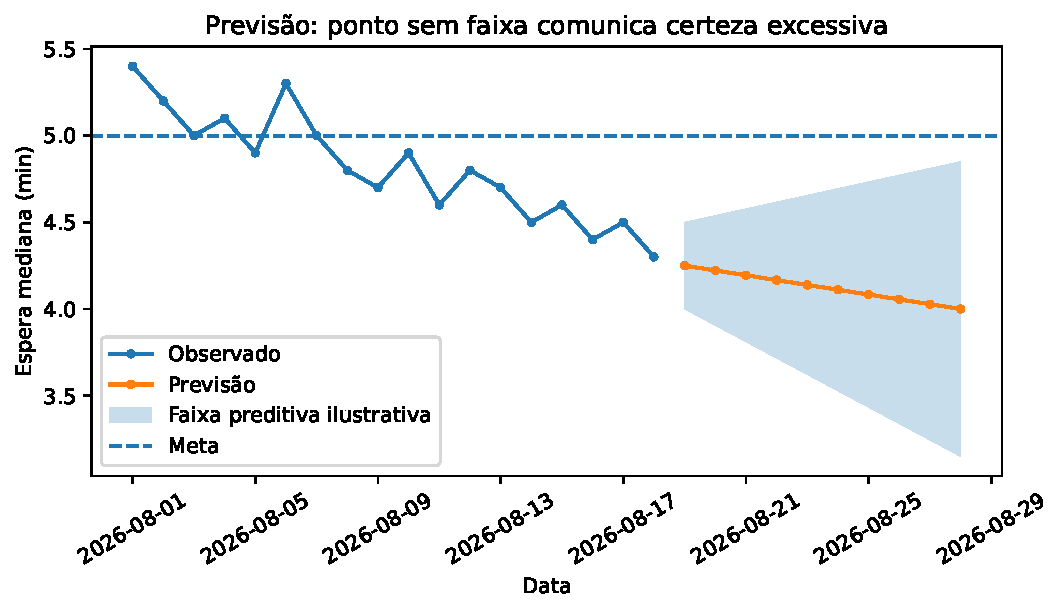
\includegraphics[width=0.84\textwidth]{fig_06_14b_previsao_intervalo.pdf}
\caption{Previsão com faixa crescente de incerteza. A faixa é ilustrativa e deve sempre ser definida pelo método que a produziu. \FonteDidatica}
\label{fig:previsao}
\end{figure}

A literatura de comunicação visual recomenda evitar precisão gráfica maior do que a evidência sustenta \cite{cairo2016,knaflic2015}. Isso vale para casas decimais, linhas pontuais de previsão, rankings com $n$ minúsculo e mapas de taxas instáveis. Uma boa figura distingue observação, estimativa, meta e previsão por marcas ou anotações, e permite que o leitor saiba qual parte foi medida e qual parte foi inferida.

\begin{GuidedBox}
\textbf{Pergunta para a turma.} Se dois intervalos de 95\% se sobrepõem, podemos concluir que não há diferença? Não automaticamente. A sobreposição visual não é um teste universal. O gráfico serve para comunicar magnitude e incerteza; a inferência depende do procedimento estatístico apropriado e da pergunta. Também precisamos distinguir relevância estatística de relevância prática.
\end{GuidedBox}


\section{Redesenho guiado e implementação reprodutível}

O redesenho começa pela afirmação. Recebemos um painel com donut de quatro turnos, barras 3D de reclamações, linha mensal em eixo duplo e mapa de atendimentos por estado. A decisão é realocar duas pessoas para reduzir espera extrema. O donut mostra participação, não risco; o 3D distorce comprimentos; o eixo duplo sugere relação; o mapa não ajuda se a escala é por turno. A primeira ação é retirar componentes sem função, não escolher uma paleta nova.

Uma versão coerente combina três vistas: pontos ordenados da mediana e P90 por turno contra a meta; pequenos múltiplos diários para verificar recorrência; tabela curta com volume, taxa e completude. O P90 representa cauda, a série revela quando e a tabela preserva denominadores. A madrugada pode exibir pior taxa, mas volume pequeno e intervalo largo. Assim, a decisão passa de ``maior barra'' para uma comparação entre severidade, frequência, confiança e capacidade.

O código vem depois do desenho conceitual e registra escolhas. Em Python, agregamos no grão turno--dia, calculamos mediana e percentil e mantemos a amostra. O mesmo raciocínio pode ser implementado em SQL e em ferramentas de BI. O importante é que campo, agregação, filtro, escala e ordenação sejam reproduzíveis. Um clique sem registro é uma transformação invisível.

\begin{verbatim}
resumo = (df.groupby("turno")["espera_min"]
            .agg(mediana="median", n="size",
                 p90=lambda s: s.quantile(.90))
            .reset_index()
            .sort_values("p90", ascending=False))

ax = resumo.plot.barh(x="turno", y="p90", legend=False,
                      color="#F28E2B")
ax.axvline(5, color="#4B5563", linestyle="--", label="meta")
ax.set(xlabel="Espera no percentil 90 (min)", ylabel="")
\end{verbatim}

O trecho não resolve sozinho qualidade, incerteza nem acesso. Antes dele, verificamos se \texttt{espera\_min} usa a mesma definição em todos os canais, se cancelamentos entram no denominador e se ausências estão distribuídas por turno. Depois dele, conferimos valores contra uma tabela, testamos filtros e registramos fonte e data de atualização. A figura é o fim visível de uma cadeia de evidência.

Faça o teste do relance: em poucos segundos, um colega consegue dizer qual é a mensagem, a unidade e a exceção? Em seguida, faça o teste de auditoria: ele consegue descobrir período, população, agregação, filtros, fonte e limite? O primeiro protege atenção; o segundo protege confiança. Uma figura pode passar em um e falhar no outro. Dashboard decisório precisa dos dois.

Ferramentas oferecem recomendações automáticas, temas e inteligência generativa. Sistemas de recomendação visual também tentam formalizar regras de percepção e tarefa; uma revisão recente mostra, porém, que a literatura perceptiva é mais rica e por vezes contraditória do que um conjunto pequeno de regras automáticas \cite{zeng2023}. Elas aceleram protótipos e podem sugerir alternativas, mas frequentemente escolhem pela forma da tabela, não pela consequência da decisão. Um modelo pode gerar código correto para uma pergunta mal formulada ou um gráfico convincente sobre taxa somada. Use automação para produzir candidatos; use contrato, percepção e domínio para aprovar a versão publicada.



O redesenho final deve ser mostrado como um \textbf{conjunto de vistas complementares}, e não como tentativa de empilhar tudo em um único gráfico. A Figura~\ref{fig:painel-mediana-p90} usa pontos para responder ``qual turno combina pior experiência típica e pior cauda?''. A série temporal já mostrada na Figura~\ref{fig:serie-temporal} responde ``quando isso acontece?''. A tabela de volume e taxa responde ``qual é o denominador e a capacidade envolvida?''. Esse é um exemplo de gráficos combinando: cada vista mantém uma tarefa clara e o conjunto sustenta a decisão.

\begin{figure}[H]
\centering
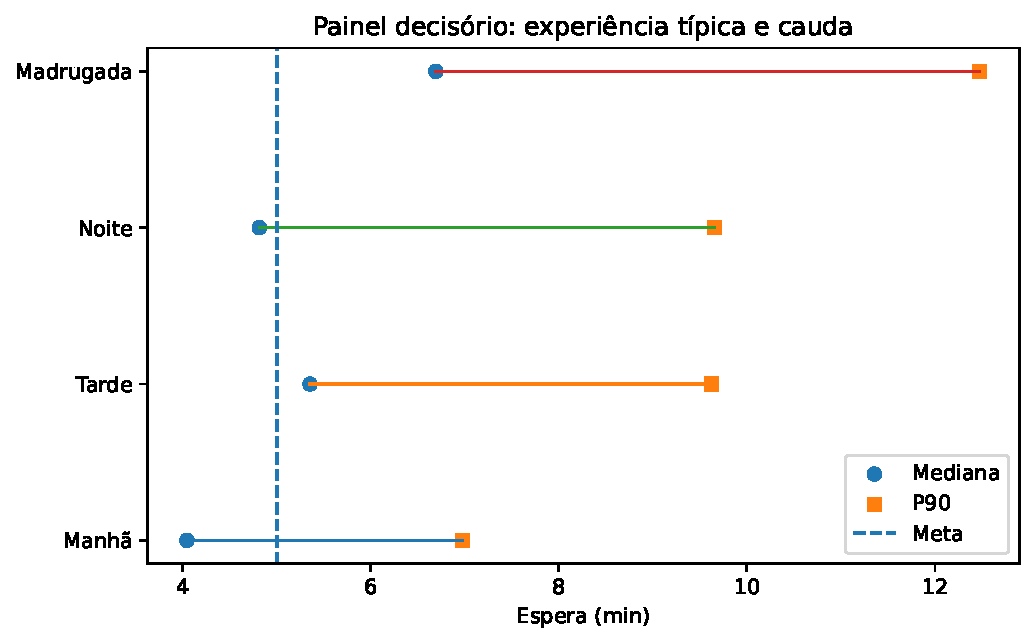
\includegraphics[width=0.84\textwidth]{fig_06_15_mediana_p90.pdf}
\caption{Painel decisório principal: mediana e P90 por turno contra a meta. A distância entre os pontos resume o quanto a cauda se afasta da experiência típica. \FonteDidatica}
\label{fig:painel-mediana-p90}
\end{figure}

\begin{center}
\small
\begin{tabular}{lrrrr}
\toprule
Turno & Atendimentos & Mediana (min) & P90 (min) & Taxa de reclamação \\
\midrule
Manhã & 2.225 & 4,05 & 6,98 & 1,93\% \\
Tarde & 1.639 & 5,35 & 9,62 & 2,75\% \\
Noite & 1.042 & 4,82 & 9,66 & 3,07\% \\
Madrugada & 424 & 6,69 & 12,48 & 7,78\% \\
\bottomrule
\end{tabular}
\end{center}

A leitura integrada muda a decisão. A manhã tem maior volume e experiência típica abaixo da meta; a madrugada tem menor volume, mas mediana, P90 e taxa de reclamação mais altos. A tarde fica ligeiramente acima da meta na mediana e possui cauda relevante. Se existem apenas duas pessoas para realocar, o gráfico não determina sozinho a solução; ele indica onde investigar capacidade, perfil da demanda, custo de cobertura e estabilidade do padrão. Essa é a diferença entre dashboard que exibe números e visualização que sustenta decisão.

Para tornar o processo reprodutível, registre não apenas o código final, mas a transformação que o antecede: grão, filtros, métricas, ordenação, limites de eixo, referência e tratamento de ausentes. O exemplo de código já existente nesta seção é mantido porque mostra a geração de um resumo e de um gráfico. O passo adicional é comparar o resultado com uma tabela independente e registrar a pergunta que justificou a escolha. Esse raciocínio aproxima visualização da ideia de ``design verificável'' defendida por obras de referência da área \cite{munzner2014,wilke2019,knaflic2015}.

\begin{GuidedBox}
\textbf{Como usar IA/LLM sem terceirizar a análise.} Um modelo pode receber a pergunta, o dicionário de dados e um resumo e sugerir três gráficos candidatos, gerar código Matplotlib/Power BI e apontar riscos. Depois peça uma segunda etapa: ``critique seu próprio gráfico quanto a escala, denominador, agregação, causalidade, acessibilidade e incerteza''. A IA acelera alternativas e implementação; a aprovação continua dependente do contrato de dados e da decisão humana.
\end{GuidedBox}


\section{Roteiro de decisão e fechamento}

A primeira etapa é escrever pergunta e ação. ``Qual turno requer intervenção na próxima escala?'' define comparação e consequência. Depois, confirme unidade de análise, população, período e métricas. Uma pergunta sobre experiência exige distribuição ou percentis, não apenas média. Uma pergunta sobre carga exige contagem; uma pergunta sobre risco pede taxa. Sem esse contrato, nenhuma escolha gráfica é estável.

A segunda etapa é classificar a operação perceptiva. Comparação favorece posição e comprimento em base comum; tendência favorece posição ao longo do tempo; distribuição pede histograma, pontos ou resumos de quantis; relação pede duas posições; composição pede partes de um total explícito. Casos reais combinam operações, mas cada painel deve ter função principal. Se um gráfico tenta responder tudo, normalmente não responde nada com clareza.

A terceira etapa é auditar escalas e canais. Verifique zero em barras, transformação, limites, unidade, denominador, ordenação e continuidade. Pergunte se área, ângulo ou cor estão sendo usados quando posição seria mais precisa. Examine como o desenho se comporta com filtros, valores ausentes, negativos e extremos. Uma escolha segura no conjunto completo pode tornar-se enganosa em um recorte interativo.

A quarta etapa é incorporar contexto e incerteza. Metas, linhas de referência, tamanho da amostra, intervalos, eventos e notas devem apoiar a afirmação sem ocupar o centro visual. Destaque apenas o que merece atenção e mantenha alternativa acessível. Depois, valide números contra fonte independente e peça a outra pessoa que descreva o que entendeu. Se a descrição divergir da pergunta, a representação falhou como comunicação.

Em uma aula de três horas, este percurso pode ser vivido em dois movimentos de noventa minutos. O primeiro vai do caso inicial às operações de comparação, tendência e distribuição, com cálculo de razões, percentis e efeito de eixo. O segundo percorre relação, composição, escalas, cor, múltiplos painéis e incerteza, terminando no redesenho da central. O ritmo alterna leitura, cálculo manual, inspeção visual e reprodução em código, sempre retomando a decisão.

O gráfico final não é ``o mais bonito'' nem ``o recomendado pelo software''. É aquele cuja gramática torna a comparação necessária direta, preserva denominadores, expõe escala e limita a inferência ao que os dados sustentam. No caso da central, o cumprimento da mediana deixa de encerrar a conversa: P90, turnos, dias, volume e incerteza mostram onde a experiência falha e quão segura é a intervenção. Visualizar bem é reduzir a distância entre evidência e decisão sem esconder o caminho.

A leitura crítica pode ser condensada em cinco perguntas repetíveis: o que cada marca representa; qual transformação liga o dado à marca; que comparação o desenho favorece; que contexto foi removido; e qual decisão mudaria se a escala, o período ou o denominador mudasse? Aplicadas antes da publicação, elas funcionam como revisão. Aplicadas a gráficos de jornal, relatórios e respostas geradas por IA, funcionam como defesa contra persuasão visual indevida. O aluno deixa de apenas consumir imagens e passa a reconstruir seus argumentos.

Essa reconstrução deve chegar até o dado. Ao encontrar um pico, procure a linha ou o agregado que o produziu; ao encontrar uma cor extrema, leia a legenda; ao encontrar um ranking, confira empates, filtros e amostra. A habilidade não é desconfiar de toda figura, mas distinguir síntese legítima de simplificação enganosa. Quando pergunta, cálculo, codificação e limite permanecem conectados, o gráfico pode ser conciso sem ser superficial e persuasivo sem manipular.

Uma entrega profissional registra também as alternativas rejeitadas. Anotar que o setor foi trocado por barras para favorecer comparação, que a média foi acompanhada pelo P90 para expor a cauda e que o eixo duplo foi separado em painéis torna o raciocínio revisável. Esse pequeno histórico funciona como decisão de projeto visual: outro analista consegue entender o propósito, testar o resultado com novos dados e reverter a escolha se a pergunta mudar. A qualidade não reside apenas na imagem final, mas na capacidade de explicar por que ela representa melhor a evidência disponível.

\begin{SummaryBox}
\textbf{Síntese.} Pergunta $\rightarrow$ operação perceptiva $\rightarrow$ marcas e canais $\rightarrow$ escala $\rightarrow$ contexto e incerteza $\rightarrow$ validação. Ferramenta é a última escolha dessa cadeia.
\end{SummaryBox}


Antes da síntese final, transforme o capítulo em um roteiro de escolha que possa ser aplicado a qualquer conjunto de dados. O processo abaixo é deliberadamente mais importante do que decorar uma lista de gráficos.

\begin{center}
\small
\begin{tabularx}{0.96\textwidth}{p{1.15cm} p{3.15cm} X}
\toprule
\textbf{Passo} & \textbf{Pergunta} & \textbf{Decisão visual} \\
\midrule
1 & O que preciso decidir? & escreva a pergunta e a ação; elimine métricas que não participam dela \\
2 & Qual é o grão e o tipo das variáveis? & confirme unidade de análise, categorias, números, tempo, geografia e denominadores \\
3 & Qual operação o leitor fará? & comparação, tendência, distribuição, relação, composição, padrão espacial/matricial ou incerteza \\
4 & Qual canal torna a tarefa mais precisa? & prefira posição/comprimento para comparação exata; use área, ângulo, cor e tamanho quando a tarefa tolerar menor precisão ou exigir outra estrutura \\
5 & Que contexto é indispensável? & meta, período, $n$, evento, fonte, filtro, unidade, denominador e incerteza \\
6 & O desenho pode enganar sem querer? & audite eixo, escala, ordem, cor, dupla escala, suavização, ausentes e interação \\
7 & A mensagem sobrevive à auditoria? & confira contra a tabela e peça a outra pessoa para descrever o que entendeu \\
\bottomrule
\end{tabularx}
\end{center}

Em termos de referências, este capítulo combina quatro tradições complementares. Cleveland e McGill estabeleceram uma base experimental para percepção gráfica, posteriormente replicada e ampliada por estudos como Heer e Bostock e revisões recentes \cite{cleveland1984,heer2010,zeng2023}. Wilkinson formalizou a gramática que separa dados, transformações, escalas e elementos geométricos \cite{wilkinson2005}. Munzner organiza o projeto em termos de dados, tarefas, marcas, canais e validação \cite{munzner2014}. Obras orientadas à prática, como Wilke, Few, Cairo e Knaflic, traduzem esses fundamentos em decisões recorrentes de comunicação e projeto \cite{wilke2019,few2012,cairo2016,knaflic2015}.

A consequência pedagógica é simples: não ensine ``pizza é ruim'' ou ``linha é boa''. Ensine a perguntar qual tarefa o gráfico precisa tornar mais fácil. Um setor com três partes muito diferentes pode comunicar composição rapidamente; quatro barras serão melhores quando a comparação exata entre partes importa. Uma linha com eixo ampliado pode ser apropriada para variação fina; uma barra truncada pode distorcer magnitude. Um heatmap pode revelar concentração em hora e dia; uma tabela é superior quando a pessoa precisa recuperar um valor exato. O contexto decide qual vantagem perceptiva é relevante.

\begin{SummaryBox}
\textbf{Mapa mental definitivo.} \textbf{Pergunta} $\rightarrow$ \textbf{grão e variável} $\rightarrow$ \textbf{operação perceptiva} $\rightarrow$ \textbf{gráfico candidato} $\rightarrow$ \textbf{escala e contexto} $\rightarrow$ \textbf{incerteza e acessibilidade} $\rightarrow$ \textbf{validação} $\rightarrow$ \textbf{decisão}. Se a ferramenta escolhe o gráfico antes dessas etapas, trate a recomendação como rascunho, não como resposta.
\end{SummaryBox}




\clearpage
\section*{Referências bibliográficas}
\addcontentsline{toc}{section}{Referências bibliográficas}
\begin{thebibliography}{99}

\bibitem{anscombe1973}
ANSCOMBE, F. J. Graphs in Statistical Analysis. \textit{The American Statistician}, v. 27, n. 1, p. 17--21, 1973. DOI: 10.1080/00031305.1973.10478966.

\bibitem{cairo2016}
CAIRO, Alberto. \textit{The Truthful Art: Data, Charts, and Maps for Communication}. Berkeley: New Riders, 2016.

\bibitem{cleveland1984}
CLEVELAND, William S.; MCGILL, Robert. Graphical Perception: Theory, Experimentation, and Application to the Development of Graphical Methods. \textit{Journal of the American Statistical Association}, v. 79, n. 387, p. 531--554, 1984. DOI: 10.1080/01621459.1984.10478080.

\bibitem{few2012}
FEW, Stephen. \textit{Show Me the Numbers: Designing Tables and Graphs to Enlighten}. 2. ed. El Dorado Hills: Analytics Press, 2012.

\bibitem{heer2010}
HEER, Jeffrey; BOSTOCK, Michael. Crowdsourcing Graphical Perception: Using Mechanical Turk to Assess Visualization Design. In: \textit{Proceedings of CHI 2010}. New York: ACM, 2010. p. 203--212. DOI: 10.1145/1753326.1753357.

\bibitem{knaflic2015}
KNAFLIC, Cole Nussbaumer. \textit{Storytelling with Data: A Data Visualization Guide for Business Professionals}. Hoboken: Wiley, 2015. DOI: 10.1002/9781119055259.

\bibitem{munzner2014}
MUNZNER, Tamara. \textit{Visualization Analysis and Design}. Boca Raton: CRC Press, 2014.

\bibitem{ware2021}
WARE, Colin. \textit{Information Visualization: Perception for Design}. 4. ed. Cambridge, MA: Morgan Kaufmann, 2021.

\bibitem{wilke2019}
WILKE, Claus O. \textit{Fundamentals of Data Visualization}. Sebastopol: O'Reilly Media, 2019.

\bibitem{wilkinson2005}
WILKINSON, Leland. \textit{The Grammar of Graphics}. 2. ed. New York: Springer, 2005. DOI: 10.1007/0-387-28695-0.

\bibitem{zeng2023}
ZENG, Zehua; BATTLE, Leilani. A Review and Collation of Graphical Perception Knowledge for Visualization Recommendation. In: \textit{Proceedings of CHI 2023}. New York: ACM, 2023. art. 820, p. 1--16. DOI: 10.1145/3544548.3581349.

\end{thebibliography}
